\documentclass[12pt]{article}
\usepackage{amsfonts}
\usepackage{listings}
\usepackage{amsmath}
\usepackage{amsthm}
\usepackage{algorithmicx}
\usepackage{algpseudocode}
\usepackage{graphicx}
\usepackage{tikz}
\usepackage{float}
\pagestyle{myheadings}
\usepackage{verbatim}
%\widowpenalties 1 10000

\author{Peter Ahrens, Hong Diep Nguyen, James Demmel}
\title{ReproBLAS: Much Summation! So Reproducible!}
\providecommand{\R}{\ensuremath{\mathbb{R}}}
\providecommand{\F}{\ensuremath{\mathbb{F}}}
\providecommand{\Z}{\ensuremath{\mathbb{Z}}}
\providecommand{\exp}{\ensuremath{\text{exp}}}
\providecommand{\min}{\ensuremath{\text{min}}}
\providecommand{\max}{\ensuremath{\text{max}}}
\providecommand{\ulp}{\ensuremath{\text{ulp}}}
\providecommand{\ufp}{\ensuremath{\text{ufp}}}
\providecommand{\fl}{\ensuremath{\text{fl}}}
\providecommand{\To}{\ensuremath{\text{ to }}}
\newcommand{\fct}[1]{\ensuremath{\mathtt{#1}}}
\providecommand{\roundtonearestinfty}{\ensuremath{\mathcal{R}_\text{$\infty$}}}
\theoremstyle{definition}
\newtheorem{thm}{Theorem}[section]
\newtheorem{lem}[thm]{Lemma}
\newtheorem{alg}{Algorithm}[section]
\numberwithin{equation}{section}
\numberwithin{figure}{section}

\graphicspath{{plots}}
\begin{document}
\noindent
\maketitle
\tableofcontents
\newpage

\section{Introduction}
  Reproducibility is important for several reasons. Primarily, bitwise identical results are useful and sometimes required for testing and debugging. It is difficult to write tests for a function when the output of the function is not well-defined. Debugging a program becomes very difficult when runs with errors cannot be examined because they cannot be reproduced \cite{reproducibilityBOF}.

  Reproducibility is also important in normal, correct operations of programs. Simulations looking rare events must be reproducible so that when a rare event is found it may be replayed and studied in more detail. Similarly, forward unstable simulations (such as N-body simulation or climate and weather modeling) must be reproducible as small changes at initial time steps can lead to big changes at later time steps. Reproducibility may also be required for contractual reasons, when multiple parties must agree on the result of a simulation (examples include finite element simulations of structures and multiplayer gaming). This is a concern in the independent verification of a published result. There have been numerous meetings at recent Supercomputing conferences addressing the need for, and proposed ways to achieve reproducibility \cite{reproducibilityBOF}.

  %note: an alternate definition of reproducibility can be used here. We can say that a procedure that computes the result of some function is "reproducible" if the procedure produces equivalent results when the function does.
  At this point is is important to define clearly what we mean by reproducibility. A computation is \textbf{reproducible} if it achieves bitwise identical results from the same computation when given equivalent inputs. The term ``equivalent inputs'' is intentionally vague, as what constitutes equivalence of inputs depends on the context and computation in question. In this work, we focus on equivalence under the associativity of addition (as this tends to be a significant source of non-reproducibility in many computations). 

  Some developers have already promised flavors of numerical reproducibility. The Intel\textregistered Math Kernel Library (MKL) introduced a feature called Conditional Numerical Reproducibility (CNR) in version 11.0 \cite{MKL}. When enabled, the code returns the same results from run-to-run as long as calls to MKL come from the same executable and the number of computational threads used by MKL is constant. Performance is degraded by these features by at most a factor of 2. However, these routines cannot offer reproducible results if the data ordering or the number of processors changes.
  %A computation is \textbf{completely reproducibile} if it produces bitwise identical output when given any two inputs equivalent up to permutation with regard to the associativity of addition. A computation is \textbf{block reproducible} if it produces bitwise identical output given any

  Reproducibility is not the same as accuracy, but they are related. Increasing the accuracy of a computation can reduce the probability of nonreproducibility, but it does not guarantee reproducibility, especially for ill-conditioned inputs or when the result is half-way between two floating point numbers in the output precision (the well-known Table Maker's Dilemma)\cite{taufer}. Ill-conditioned inputs (e.g., a tiny sum resulting from extensive cancellation) may be the most common case in many applications. For example, when solving $Ax = b$ using an iterative method, the goal is to get as much cancellation in the residual $r = Ax - b$ as possible.

  With these considerations in mind, reproducible algorithms for summations were presented in \cite{repsum}. The algorithms were shown to enjoy the following properties:
  \begin{enumerate}
    \item They compute a reproducible sum independent of the order of the summands, how they are assigned to processors, or how they are aligned in memory.
    \item They make only basic assumptions about the underlying arithmetic (a subset of IEEE Standard 754-2008 \cite{ieee754}).
    \item They scale as well as a performance-optimized, non-reproducible implementation, as $n$ (number of summands) and $p$ (number of processors) grow, performing one pass over the data, and requiring just one reduction operation in the parallel case.
    \item The user can choose the desired accuracy of the result. In particular, getting a reproducible result with about the same accuracy as the performance optimized algorithm is only a small constant times slower, but higher accuracy is possible too.
  \end{enumerate}
  The algorithms of \cite{repsum} did not, however, work for all ranges of floating-point input (because of over/underflow) nor did they contain all of the functional components necessary to be deployed in an existing application (they lacked an algorithm to convert from a reproducible type back to floating point format while maintaining accuracy).
   We have improved the error bound of \cite{repsum} by over 8 orders of magnitude in a typical configuration, as discussed in Section \ref{sec:primitiveops_conv2float}. Our goal is to modify the algorithms in \cite{repsum} so that in addition to the above properties, they enjoy the following properties:
  \begin{enumerate}
    \item The algorithms can be applied in any binary IEEE 754-2008 floating point format, and any valid input in such a format can be summed using the algorithms. The algorithms must be able to reproducibly sum numbers numbers close to underflow or overflow, and exceptional values such as \texttt{NaN} and \texttt{Inf}, mimicking the behavior of IEEE floating point wherever possible.
    \item The algorithms must be expressed in terms of basic operations that can be applied in several applications. They must be able to be built into a user-friendly, performant library. This includes the ability to produce a floating-point result of comparable accuracy to the (intermediate) reproducible type.
  \end{enumerate}

We summarize the algorithm informally as follows.
The simplest approach would be to
\begin{enumerate}
\item compute the maximum absolute value $M$ of all the
summands (this is exact and so reproducible),
\item round all the summands to 1 ulp (unit in the last
place) of $M$ (this introduces error, but not worse than
the usual error bound), and then
\item add the rounded summands (since their nonzero bits
are aligned, they behave like fixed point numbers, so
summation is exact and so reproducible, assuming we
have $\log_2 n$ extra bits for carries).
\end{enumerate}
The trouble with this simple approach is that it requires
2 or 3 passes over the data, or 3 communication steps in parallel.
We can in fact do it in one pass over the data, or one communication
step, essentially by interleaving the 3 steps above:
We break the floating point exponent range into fixed \textbf{bins} all of
some width $W$ (see Figure \ref{fig:binning}). Each summand is then rewritten as the
exact sum of a small number of \textbf{slices}, where each slice corresponds
to the significant bits of the summand lying (roughly) in a bin. We can then sum
all slices corresponding the same bin exactly, again because we are
(implicitly) doing fixed point arithmetic.  But we do not need
to sum the slices in all bins, only the bins corresponding to the largest
few exponent ranges (the number of bins summed can be chosen based on
the desired precision). Slices lying in bins with smaller exponents are
discarded or not computed in the first place. Independent of the order
of summation, we end up with the same sums of slices in the same bins, all computed exactly and
so reproducibly, which we then convert to a standard floating point number.
As we will see, this idea, while it sounds simple, requires significant effort
to implement and prove correct.

  Section \ref{sec:notation} begins by explaining some of the notation necessary to express the mathematical and software concepts discussed in this work.
  Section \ref{sec:binning} gives a formal discussion of the binning scheme. As described above, a floating point number $x$ is split along predefined boundaries (bins) into a sum of separate numbers (slices) such that the sum of slices equals (or approximates) $x$. We sum the slices corresponding to each bin separately and exactly.
  Section \ref{sec:indexed} describes the data structure (the \textbf{indexed type}) used to store the sums of the slices.
  Section \ref{sec:primitiveops} contains several algorithms for basic manipulations of an indexed type.  These algorithms allow the user to, for instance, extract the slices of a floating point number and add them to the indexed type, to add two indexed types together, or to convert from the indexed type to a floating point number. We show that the absolute error of the reproducibly computed sum of double-precision floating point numbers $x_0, ..., x_{n - 1}$ in a typical use case is bounded by
  \[
    n 2^{-80} \max|x_j| + 7 \epsilon|\sum\limits_{j = 0}^{n - 1} x_j|
  \]
  Details regarding the error bound are given in Sections \ref{sec:primitiveops_conv2float} and \ref{sec:primitiveops_error}.
  As discussed in Section \ref{sec:primitiveops_restrictions}, the indexed types are capable of summing approximately $2^{64}$ \texttt{double}s or $2^{33}$ \texttt{float}s.
  Section \ref{sec:compositeops} gives several descriptions of algorithms that can be built from the basic operations described in Section \ref{sec:primitiveops}. In particular, several sequential reproducible algorithms from the BLAS (Basic Linear Algebra Subprograms) are given.
  Throughout the text, relevant functions from ReproBLAS (the C library accompanying this work from which these algorithms are taken) are mentioned. The interfaces to these functions allow the user to adjust the accuracy of the indexed types used. ReproBLAS uses a custom build system, code generation, and autotuning to manage the software engineering complexities of performance-optimized code. A short description of ReproBLAS, including timing data and testing methods, is given in Section \ref{sec:reproBLAS}. ReproBLAS is available online at \path{http://bebop.cs.berkeley.edu/reproblas}.

\section{Notation and Background}
  Let $\R$ and $\Z$ denote the sets of real numbers and integers respectively.

  For all $r \in \R$, let $r\Z$ denote the set of all multiples of $r$,
  $\{rz | z \in \Z\}$.

  For all $r \in \R$, let $\lceil r \rceil$ be the minimum element $z \in \Z$
  such that $z \geq r$.

  For all $r \in \R$, let $\lfloor r \rfloor$ be the maximum element $z \in \Z$
  such that $z \leq r$.

  We define the function $\roundtonearestinfty(r, e), r \in R, e \in \Z$ as

  \begin{equation}
    \roundtonearestinfty(r, e) = \begin{cases}
        \lfloor r/2^e + 1/2 \rfloor 2^e \text{ if } r \geq 0\\
        \lceil r/2^e - 1/2 \rceil 2^e \text{ otherwise}
    \end{cases}
  \end{equation}

  $\roundtonearestinfty(r, e)$ rounds $r$ to the nearest multiple of $2^e$,
  breaking ties away from 0. Properties of such rounding are shown in
  \eqref{eq:round}
  \begin{equation}
    \begin{aligned}
    \bigl|r - \roundtonearestinfty(r, e)\bigr| & \leq 2^{e - 1} \\
    \roundtonearestinfty(r,e) & = 0 \text{ if } r < 2^{e-1}.
    \end{aligned}
    \label{eq:round}
  \end{equation}

  Let $\F_{b,p,e_{min},e_{max}}$ denote the set of floating-point numbers
  of base $b \in \Z$ ($b \geq 2$),
  precision $p \in Z$ ($p \geq 1$) and exponent range $[e_{min}, e_{max}]$
  where $e_{min}, e_{max} \in \Z$ and $e_{min} \geq e_{max}$.
  Each value $f \in \F_{b,p,e_{min},e_{max}}$ is represented by:
  \[
    f = s \cdot m_0.m_1 \ldots m_{p-1} \cdot b^e,
  \]
  where $s \in \{-1,1 \}$ is the sign,
  $e \in \Z, e_{\min} \leq e \leq e_{\max}$ is the exponent
  (also defined as $exp(f)$),
  and $m = m_0.m_1 \ldots m_{p-1}, m_i \in \{ 0, 1, \ldots, b-1 \}$
  is the significand (also called the mantissa) of $f$. Assume that the
  representation of $f$ is made unique using the ``hidden bit'' convention, so
  that $f$ is represented using the smallest exponent possible.

  Although much of the below analysis can be applied to a general floating-point
  format, in the context of this paper we assume binary floating-point formats,
  i.e. $b=2$, complying with the IEEE 754-2008 standard \cite{ieee754}. 
  While the below analysis applies for any chosen values of $p$, $e_{\min}$, and $e_{\max}$ 
  (provided that $p << e_{\max} - e_{\min}$), our software is implemented in IEEE 754-2008
   single and double precision.

  Specific parameters for those two formats are given in Table \ref{tbl:IEEE-754}.
  \begin{table}[!htbp]
    \caption{IEEE 754-2008 binary floating-point formats}
    \label{tbl:IEEE-754}
        \centering
        \begin{tabular}{ | l | l | l | } \hline
            Floating-Point Type & single precision & double precision \\ \hline
            C data type & \texttt{float} & \texttt{double} \\ \hline
            $p$ & 24 & 53 \\ \hline
            Exponent field width & 8 & 12 \\ \hline
            Exponent bias & 127 & 1023 \\ \hline
            $e_{min}$ & -126 & -1022 \\ \hline
            $e_{max}$ & 127 & 1023 \\ \hline
        \end{tabular}
  \end{table}

  \begin{comment}
  Let $\F$ be the set of all floating-point numbers $f = sm2^e$ represented in some binary IEEE 754-2008 format \cite{ieee754} where $s \in \{1, -1\}$ is the \textbf{sign},
  $e \in \Z$, $e_{\max} \geq e \geq e_{\min}$ is the \textbf{exponent} ($\exp(f)$ is
  defined to be $e$), $p \in \Z, p > 1$ is the \textbf{precision},
  and $m=m_0.m_1m_2...m_{p-1}$ where $m_0, ..., m_{p - 1} \in \{0, 1\}$ is the
  \textbf{significand} of $f$. Assume that the representation of $f$ is made unique using the ``hidden bit'' convention, so that $f$ is represented using the smallest exponent possible. (In memory, the bit $m_0$ is not stored and assumed to be 1 unless the exponent field contains a special value signaling both that $e = e_{\min}$ and $m_0=0$).
  $f$ is said to be \textbf{normalized} if $m_0 =1$
  and $e \geq e_{\min}$, \textbf{unnormalized} if $m_0 = 0$, and
  \textbf{denormalized} if $m_0 = 0$ and $e = e_{\min}$. $f = 0$ if all $m_j = 0$
  and $e = e_{\min}$.

  Assume that floating point arithmetic complies with the IEEE 754-2008
  standard \cite{ieee754} in some ``to nearest'' rounding mode (no specific tie
  breaking behaviour is required) and that underflow occurs gradually, although
  methods to handle abrupt underflow will be considered in Section
  \ref{sec:indexed_underflow_abrupt}.

  Let $f = sm2^e \in \F$ be a floating-point number represented in IEEE
  754-2008 format \cite{ieee754} where $s \in \{1, -1\}$ is the \textbf{sign},
  $e_{\max} \geq e \geq e_{\min}$ is the \textbf{exponent} ($\exp(f)$ is
  defined to be $e$), $p$ is the \textbf{precision},
  and $m=m_0.m_1m_2...m_{p-1}$ where $m_0, ..., m_{p - 1} \in \{0, 1\}$ is the
  \textbf{significand} of $f$.
  \end{comment}

  The exponent is stored in internal representation in biased form
  using 8 bits for single precision, and 53 bits for double precision.
  The exponent of a represented floating-point number is equal to
  the biased exponent (the unsigned integer value stored in the exponent field)
  minus the bias value (see table~\ref{tbl:IEEE-754}).
  An exponent field with all bits set to 0 is reserved for zeros and denormalized values.
  An exponent field with all bits set to 1 is reserved for infinities and NaN.

  Since a floating point number is always represented using the smallest possible
  exponent, the first bit $m_0$ is not explicitly stored in internal representation
  and is referred to as the "hidden" or "implicit" bit.
  Therefore only $p-1$ bits are used to represent the mantissa of $f$.

  $f = 0$ if and only if all $m_j = 0$ and $e = e_{\min} - 1$.
  $f$ is said to be \textbf{normalized} if $m_0 =1$
  and $e_{max} \geq e \geq e_{\min}$.
  $f$ is said to be \textbf{unnormalized} if $m_0 = 0$ (unnormalized numbers can 
  exist if the hidden bit convention is not followed), and
  \textbf{denormalized} if $m_0 = 0$ and $e = e_{\min} - 1$.

  In binary internal representation, $f=0$ is represented by a biased exponent of $0$
  as well as a mantissa field of all 0-bits.
  Denormalized numbers have biased exponent of $0$ and non-zero mantissa field.
  An exponent field of all 1-bits and a mantissa field of all 0-bits
  represent infinities, positive or negative depending on the sign bit.
  An exponent field of all 1-bits and a non-zero mantissa field
  represent a NaN value.

  We assume rounding mode ``to nearest'' (no specific tie
  breaking behavior is required) and gradual underflow, although
  methods to handle abrupt underflow will be considered in Section
  \ref{sec:indexed_underflow_abrupt}.

  For simplicity as well as for readability, throughout this paper
  $\F_{b,p,e_{min},e_{max}}$ will be written simply as $\F$, referring to
  some IEEE 754-2008 binary floating-point format,
  i.e. $b=2$ and $m_i \in \{0, 1\}$.
  All the analysis will be based on the corresponding parameters $p$, $e_{min}$
  and $e_{max}$.

  $r \in \R$ is \textbf{representable} as a floating point number if there
  exists $f \in \F$ such that $r = f$ as real numbers.

  For all $r \in \R$, $e \in \Z$ such that $e_{\min} - p < e$ and $|r| < 2
  \cdot 2^{e_{\max}}$, if $r \in 2^e\Z$ and $|r| \leq 2^{e + p}$ then $r$ is
  representable.

  Machine epsilon, $\epsilon$, the difference between 1 and the greatest
  floating point number smaller than 1, is defined as $\epsilon = 2^{-p}$.

  The unit in the last place of $f \in \F$, $\ulp(f)$, is the spacing between
  two consecutive floating point numbers of the same exponent as $f$. If $f$ is
  normalized, $\ulp(f) = 2^{\exp(f) - p + 1} = 2  \epsilon  2^{\exp(f)}$ and
  $\ulp(f) \leq 2^{p - 1}|f|$.

  The unit in the first place of $f \in F$, $\ufp(f)$, is the value of the
  first significant bit of $f$. If $f$ is normalized, $\ufp(f) = 2^{\exp(f)}$.

  For all $f_0, f_1 \in \F$, $\fl(f_0 \text{ op } f_1)$ denotes the evaluated
  result of the expression $(f_0 \text{ op } f_1)$ in floating point
  arithmetic. If $(f_0 \text{ op } f_1)$ is representable, then
  \(
    \fl(f_0 \text{ op } f_1) = (f_0 \text{ op } f_1).
  \)
  If rounding is ``to nearest,'' then we have that
  \(
    |\fl(f_0 \text{ op } f_1) - (f_0 \text{ op } f_1)| \leq 0.5\ulp(\fl(f_0 \text{ op } f_1)).
  \)

%TODO At this point, the reader does not know what ReproBLAS is
  As ReproBLAS is written in C, \texttt{float} and \texttt{double} refer to the
  floating point types specified in the 1989 C standard \cite{c89} and we
  assume that they correspond to the \texttt{binary-32} and \texttt{binary-64}
  types in the IEEE 754-2008 floating point standard \cite{ieee754}.

  All indices start at $0$ in correspondence with the actual ReproBLAS implementation.

\section{The Indexed Type}
  \label{sec:indexed}
    The \textbf{indexed type} is used to represent the intermediate result of
    accumulation using Algorithms 6 and $7$ in \cite{repsum}.  An indexed type
    $Y$ is a data structure composed of several accumulator data structures
    $Y_0, ..., Y_{K - 1}$. An indexed type with $K$ accumulators is referred to
    as a \textbf{$K$-fold} indexed type. Due to their low accuracy, 1-fold
    indexed types are not considered.

    Let $Y$ be the indexed type corresponding to the reproducibly computed sum
    of $x_0, ..., x_{n - 1} \in \F$. $Y$ is referred to as the \textbf{indexed
    sum} of $x_0, ..., x_{n - 1}$.

    Each accumulator $Y_k$ is a data structure used to accumulate the slices of
    input in the bin $(a_{I + k}, b_{I + k}]$ where $I$ is the \textbf{index}
    of $Y$ and $k \geq 0$ as discussed below. The \textbf{width} of an indexed
    type is equal to the width of its bins, $W$. Recall the assumptions
    \eqref{eq:wupper} and \eqref{eq:wlower} made on the value of $W$.

    The accumulators in an indexed type correspond to contiguous bins in
    decreasing order. The index of $Y$ is defined as the least $I \in \Z$ such
    that $2^{b_I + 1} > \max(|x_0|, ..., |x_n|)$ (equivalently,
    the least $I \in \Z$ such that $b_I > \max(e_0, ..., e_n)$ where $e_i=\exp(x_i)$).
    If $Y$ has index $I$, then $Y_k, k \in \{0, ..., K - 1\}$ accumulates slices
    of input in the bin $(a_{I + k}, b_{I + k}]$. If $I$ is so large that
    $I + K > i_{\max}$, then the extra $I + K - i_{\min}$ accumulators are unused.

    Section \ref{sec:indexed_primary_carry} elaborates on the specific fields
    that make up the indexed type and the values they represent. Sections
    \ref{sec:indexed_overflow}, \ref{sec:indexed_underflow_gradual},
    \ref{sec:indexed_underflow_abrupt}, and \ref{sec:indexed_exceptions}
    contain extensions of the indexed type to handle overflow, underflow, and
    exceptional values.

    \subsection{Primary and Carry}
      \label{sec:indexed_primary_carry}
      As discussed in \cite{repsum}, indexed types are represented using
      floating point numbers to minimize traffic between floating point and
      integer arithmetic units.

      In the ReproBLAS library, if an indexed type is used to sum
      \texttt{doubles}, then it is composed entirely of \texttt{doubles} and
      likewise for \texttt{floats}. ReproBLAS supports complex types as pairs
      of real and imaginary components (stored contiguously in memory). If an
      indexed type is used to sum complex \texttt{doubles} or \texttt{floats},
      then it is composed of pairs (real part, imaginary part) of
      \texttt{doubles} or \texttt{floats} respectively. The decision to keep
      the real and imaginary components together (as opposed to keeping
      separate indexed types for real and imaginary parts of the sum) was
      motivated by a desire to process accumulators simultaneously with
      vectorized (SIMD) instructions.

      The accumulators $Y_k$ of an indexed type $Y$ are each implemented using
      two underlying floating point fields. The \textbf{primary} field
      ${Y_k}_P$ is used during accumulation, while the \textbf{carry} field
      ${Y_k}_C$ holds overflow from the primary field. Because primary fields
      are frequently accessed sequentially, the primary fields and carry fields
      are each stored contiguously in separate arrays. The notation for the
      primary field ${Y_k}_P$ and carry field ${Y_k}_C$ corresponds to the
      ``$S_j$'' and ``$C_j$'' of Algorithm $6$ in \cite{repsum}.

      The numerical value ${\mathcal{Y}_k}_P$ represented by data stored in the
      primary field ${Y_k}_P$ is an offset from $1.5\epsilon^{-1}2^{a_{I + k}}$
      (corresponding to ``$M_{[i]}$'' at the beginning of Section IV.A. in
      \cite{repsum}), where $I$ is the index of $Y$, as shown in
      \eqref{eq:pri} below.
      Note that \eqref{eq:pri} only holds when $I+k > 0$. The special case of $I+k=0$,
      where $1.5\epsilon^{-1}2^{a_0} > 2^{1+e_{max}}$ is not representable,
      will be handled in Section~\ref{sec:indexed_overflow} below on Overflow.
      \begin{equation}
        {\mathcal{Y}_k}_P = {Y_k}_P - 1.5\epsilon^{-1}2^{a_{I + k}}
        \label{eq:pri}
      \end{equation}
      This simplifies the process of extracting the slices of input in bins
      $(a_{I + k}, b_{I + k}]$. It will be shown in Theorem
      \ref{thm:ddepositrestricted} in Section~\ref{sec:primitiveops_deposit}
      that if we represent each primary value ${\mathcal{Y}_k}_P$ as in
      \eqref{eq:pri} and keep ${Y_k}_P$ within the range
      \(
      	(\epsilon^{-1} 2^{a_{I + k}}, 2 \epsilon^{-1} 2^{a_{I + k}}),
      \)
      then Algorithm
      \ref{alg:depositrestricted} in Section~\ref{sec:primitiveops_deposit}
      extracts the slices of $x$ in bins 
      \(
      	(a_I, b_I], \ldots, (a_{I + K - 1}, b_{I + K - 1}]
      \)
      and adds them to ${Y_0}_P, \ldots, {Y_{K - 1}}_P$ without error
      (and hence reproducibly) for all $x \in \F$, where $|x| < 2^{b_I}$.

      Because $d(x, I + k) = 0$ for bins with $|x| < 2^{a_{I + k}}$, the values
      in the greatest $K$ nonzero accumulators can be computed reproducibly by
      computing the values in the greatest $K$ accumulators needed for the
      largest $x$ seen so far. Upon encountering an $x \geq 2^{b_I}$, the
      accumulators can then be shifted towards index $0$ as necessary.  Since
      the maximum absolute value operation is always reproducible, so is the
      index of the greatest accumulator.
      %\cite{repsum} contains further discussions of the reproducibility of the algorithm.

      In order to keep the primary fields in the necessary range while the
      slices are accumulated and to keep the representation of $Y_k$ unique,
      ${Y_k}_P$ is routinely renormalized to the range 
      \(
        [1.5 \epsilon^{-1} 2^{a_{I + k}}, 1.75 \epsilon^{-1} 2^{a_{I + k}}).
      \)
      As will be shown in Section~\ref{sec:primitiveops_renormalize},
      that renormalization is required every $2^{p-W-2}$ iterations,
      so $2^{11}$ in double and $2^9$ in single precision.
      This means the renormalization introduces a very low overhead
      to the overall running time.
      %Section \ref{sec:primitiveops_renormalize} contains a discussion of how often such renormalizations are necessary.
      To renormalize, ${Y_k}_P$ is incremented or decremented by
      $0.25 \epsilon^{-1} 2^{a_{I + k}}$ as described in Algorithm~\ref{alg:renorm},
      leaving the carry field ${Y_k}_C$ to record the number of such adjustments.
      Depending on the data format used to store ${Y_k}_C$, the number of
      updates to one accumulator without overflow is limited,
      which determines the possible maximum number of inputs that can be
      reproducibly added to one accumulator.
      As will be explained in Section~\ref{sec:primitiveops_renormalize},
      Equation~\eqref{eq:totalfreq}, using the same precision $p$ as the primary field
      to store the carry field, the total number of inputs
      that can be reproducibly added to one accumulator is $2^{2p-W-2}$.
      The numerical value ${\mathcal{Y}_k}_C$ represented by data stored in the carry field
      ${Y_k}_C$ of an indexed type $Y$ of index $I$ is expressed in
      \eqref{eq:car}
      \begin{equation}
        {\mathcal{Y}_k}_C = (0.25\epsilon^{-1}2^{a_{I + k}}){Y_k}_C
        \label{eq:car}
      \end{equation}
      Combining \eqref{eq:pri} and \eqref{eq:car}, we get that the value $\mathcal{Y}_k$ of the accumulator $Y_k$ of an indexed type $Y$ of index $I$ is
      \begin{equation}
        \mathcal{Y}_k = {\mathcal{Y}_k}_P + {\mathcal{Y}_k}_C = ({Y_k}_P - 1.5 \epsilon^{-1}2^{a_{I + k}}) + (0.25\epsilon^{-1}2^{a_{I + k}}){Y_k}_C
        \label{eq:acc}
      \end{equation}
      Therefore, using  \eqref{eq:acc}, the numerical value $\mathcal{Y}$ represented by data stored in a $K$-fold indexed type $Y$ of index $I$ (the sum of $Y$'s accumulators) is
      \begin{equation}
        \mathcal{Y} = \sum\limits_{k = 0}^{K - 1} \mathcal{Y}_k = \sum\limits_{k = 0}^{K - 1} \bigl(({Y_k}_P - 1.5 \epsilon^{-1}2^{a_{I + k}}) + (0.25\epsilon^{-1}2^{a_{I + k}}){Y_k}_C\bigr)
        \label{eq:indexedvalue}
      \end{equation}
      It is worth noting that by keeping ${Y_k}_P$ within the range
      \(
      	(\epsilon^{-1} 2^{a_{I + k}}, 2 \epsilon^{-1} 2^{a_{I + k}})
      \)
      for $I+k > 0$, the exponent of ${Y_0}_P$ is $a_I + p$ when $I > 0$.
      The case of $I = 0$ will be explained in the below section of Overflow.
      Therefore it is unnecessary to store the index of an indexed type explicitly.
      As will be explained in
      Section~\ref{sec:primitiveops_index}, the index can be determined by
      simply examining the exponent of ${Y_0}_P$, as all $a_I$ are distinct and
      the mapping between the exponent of ${Y_0}_P$ and the index of $Y$ is
      bijective.

    \subsubsection{Overflow}
      \label{sec:indexed_overflow}
      If an indexed type $Y$ has index 0 and the width is $W$, then the value
      in the primary field ${Y_0}_P$ would be stored as an offset from
      $1.5\epsilon^{-1}2^{e_{\max} + 1 - W}$. However,
      \(
        1.5\epsilon^{-1}2^{e_{\max} + 1 - W} > 2^{e_{\max} + 1 + (p - W)}
            > 2 \cdot 2^{e_{\max}}
      \) since $W < p - 2$, so it would be out of the range of the
      floating-point system and not representable. Before discussing the
      solution to this overflow problem, take note of Theorem
      \ref{thm:overflow}.

      \begin{samepage}
      \begin{thm}
        If $2 W > p + 1$, then for any indexed type $Y$ of index $I$ and any ${Y_k}_P$ such that $I + k \geq 1$, $|{Y_k}_P| < 2^{e_{\max}}$.
        \label{thm:overflow}
      \end{thm}
    \end{samepage}

      \begin{proof}
        $a_1 = e_{\max} + 1 - 2 W$ by \eqref{eq:a}, therefore $a_1 < e_{\max} - p$ using $2W > p+1$ and since all quantities are integers, $a_1 \leq e_{\max} - p - 1$. If $I + k \geq 1$, $a_{I + k} \leq a_1 \leq e_{\max} - p - 1$ by \eqref{eq:a}.

        ${Y_k}_P$ is kept within the range $(\epsilon^{-1} 2^{a_{I + k}}, 2 \epsilon^{-1} 2^{a_{I + k}})$, therefore
        \begin{equation*}
          |{Y_k}_P| < 2 \epsilon^{-1} 2^{a_{I + k}} \leq 2^{1 + p} 2^{e_{\max} - 1 - p} = 2^{e_{\max}}
        \end{equation*}
      \end{proof}
      By Theorem \ref{thm:overflow}, if $2 W > p + 1$ then the only primary
      field that could possibly overflow is a primary field corresponding to
      bin 0, and all other primary fields have exponent less than $e_{\max}$.
      Therefore, we require $2 W > p + 1$ and express the value of the primary
      field corresponding to bin 0 as a scaled offset from
      $1.5\cdot2^{e_{\max}}$. Note that this preserves uniqueness of the
      exponent of the primary field corresponding to bin 0 because no other
      primary field has an exponent of $e_{\max}$. The value
      ${\mathcal{Y}_0}_P$ stored in the primary field ${Y_0}_P$ of an indexed
      type $Y$ of index 0 is expressed in \eqref{eq:pri0}.
      \begin{equation}
        {\mathcal{Y}_0}_P = 2^{p - W + 1}({Y_0}_P - 1.5\cdot2^{e_{\max}})
        \label{eq:pri0}
      \end{equation}
    \subsubsection{Gradual Underflow}
      \label{sec:indexed_underflow_gradual}
      Here we consider the effects of gradual underflow on algorithms described
      in \cite{repsum} and how the indexed type allows these algorithms to work
      correctly.

    \label{sec:primitiveops_deposit}
      Algorithms \ref{alg:deposit} for adding a floating point input to an
      indexed type in Section~\ref{sec:primitiveops_deposit} and
      Algorithm~\ref{alg:renorm} for renormalizing an indexed type in
      Section~\ref{sec:primitiveops_renormalize} require that the primary
      fields ${Y_k}_P$ are normalized to work correctly. Theorem
      \ref{thm:underflowufp} shows that the primary fields should always be
      normalized.

      \begin{samepage}
      \begin{thm}
        For any primary field ${Y_k}_P$ of an indexed type $Y$ of index $I$ where ${Y_k}_P \in (\epsilon^{-1} 2^{a_{I + k}}, 2 \epsilon^{-1} 2^{a_{I + k}})$ (${Y_0}_P \in (2^{e_{\max}}, 2 \cdot 2^{e_{\max}})$ if $Y$ has index 0), ${Y_k}_P$ is normalized.
        \label{thm:underflowufp}
      \end{thm}
      \end{samepage}

      \begin{proof}
        By \eqref{eq:binmin},
        \begin{equation*}
        a_{I + k} \geq a_{i_{\max}} = e_{\min} - p + 2 + \bigl((e_{\max} - e_{\min} + p - 1) \mod W\bigr) \geq e_{\min} - p + 2
        \end{equation*}

        Because ${Y_k}_P \in (\epsilon^{-1} 2^{a_{I + k}}, 2 \epsilon^{-1} 2^{a_{I + k}})$ we have $\exp({Y_k}_P) = a_{I + k} + p > e_{\min} + 1$ so ${Y_k}_P$ is normalized.
      \end{proof}

      Algorithms \ref{alg:depositrestricted} and \ref{alg:deposit} rely on
      setting the last bit of intermediate results before adding them to
      ${Y_k}_P$ in order to fix the direction of the rounding mode. However, if
      $r$ is the quantity to be added to ${Y_k}_P$, $\ulp(r)$ must be less than
      rounding error when added to ${Y_k}_P$.
      Mathematically, we will require $\ulp(r) < 0.5\ulp({Y_k}_P)$ in order to
      prove Theorem~\ref{thm:ddeposit} about the correctness of
      Algorithm~\ref{alg:deposit}.  This is why we must enforce $a_{i_{\max}}
      \geq e_{\min} - p + 2$ so that the least significant bit of the least bin
      is larger than twice the smallest denormalized number.

      Although the bins do not extend all the way to $e_{\min} - p$, we now
      show that the sum of the slices of some $x \in \F$ still offers a good
      approximation of $x$.

      Using $W < p - 2$ and \eqref{eq:binmin},
      \begin{align*}
        a_{i_{\max}} & = e_{\min} - p + 2 + \bigl((e_{\max} - e_{\min} + p - 1 ) \mod W \bigr) \\
            & \leq e_{\min} - p + 2 + (W - 1) \\
            & < e_{\min} - p + 2 + (p - 2 - 1) =  e_{\min} - 1 
      \end{align*}

      Hence,
      \[
        a_{i_{\max}} \leq e_{\min} - 2
      \]

      As a consequence, we can use Theorem \ref{thm:dround} to say that for any $x \in \F$,
      \begin{equation}
        \bigl|x - \sum\limits_{i = 0}^{i_{\max}} d(x, i)\bigr| \leq 2^{a_{i_{\max}}} \leq 2^{e_{\min} - 2}
        \label{eq:droundunderflow}
      \end{equation}

      This means that we can approximate $x$ using the sum of its slices to the
      nearest multiple of $2^{e_{\min}-1}$.

      It is possible to sum the input in the denormalized range. One simple way
      the algorithm could be extended to denormalized inputs would be to scale
      the least bins up, analogously to the way we handled overflow. Due to the
      relatively low priority for accumulating denormalized values, this method
      was not implemented in ReproBLAS.

    \subsubsection{Abrupt Underflow}
      \label{sec:indexed_underflow_abrupt}
      If underflow is abrupt, several approaches may be taken to modify the
      given algorithms to ensure reproducibility.

      The most straightforward approach would be to accumulate input in the
      denormalized range by scaling the smaller inputs up. This has the added
      advantage of increasing the accuracy of the algorithm. A major
      disadvantage to this approach is the additional branching cost incurred
      due to the conditional scaling.

      A more efficient way to solve the problem would be to set the least bin
      to have $a_{i_{\max}} = e_{\min}$. This means that all the values smaller
      than $2^{e_{\min}}$ will not be accumulated,
      i.e. similarly to zeroing out the mantissa bits of each summand
      that correspond to values $2^{(e_min-1)}$ or smaller.
      This could be accomplished either
      by keeping the current binning scheme and having the least bin be of a
      width not necessarily equal to $W$, or by shifting all other bins to be
      greater. The disadvantage of shifting the other bins is that it may cause
      multiple greatest bins to overflow, adding multiple scaling cases.
      Setting such a least bin would enforce the condition that no underflow
      occurs since all intermediate sums are either $0$ or greater than the
      underflow threshold. The denormal range would be discarded.

      In the case that reproduciblity is desired on heterogeneous machines,
      where some processors may handle underflow gradually and others abruptly,
      the approach of setting a least bin is recommended. The indexed sum using
      this scheme does not depend on whether or not underflow is handled
      gradually or abruptly, so the results will be the same regardless of
      where they are computed.

    \subsubsection{Exceptions}
      \label{sec:indexed_exceptions}
      Indexed types are capable of representing exceptional cases such as
      \texttt{NaN} (Not a Number) and \texttt{Inf} (Infinity). An indexed type
      $Y$ stores its exception status in its first primary field ${Y_0}_P$.

      A value of $0$ in ${Y_0}_P$ indicates that nothing has been added to
      ${Y_0}_P$ yet (${Y_0}_P$ is initialized to $0$).

      Since the ${Y_k}_P$ are kept within the range
      \(
      	(\epsilon^{-1}  2^{a_{I + k}}, 2 \epsilon^{-1} 2^{a_{I + k}})
      \) (where $I$ is the index) and are
      normalized (by Theorem \ref{thm:underflowufp}), we have

      \begin{equation*}
        {Y_k}_P > 2^{e_{\min}}
      \end{equation*}

      Therefore the value of $0$ in a primary field is unused in any previously
      specified context and may be used as a sentinel value. (As the exponent
      of $0$ is distinct from the exponent of normalized values, the bijection
      between the index of an indexed type $Y$ and the exponent of ${Y_0}_P$ is
      preserved)

      A value of \texttt{Inf} or \texttt{-Inf} in ${Y_0}_P$ indicates that one or more \texttt{Inf} or \texttt{-Inf} (and no other exceptional values) have been added to $Y$ respectively.

      A value of \texttt{NaN} in ${Y_0}_P$ indicates that one or more \texttt{NaN}s have been added to $Y$ or one or more of both \texttt{Inf} and \texttt{-Inf} have been added to $Y$.

      As the ${Y_k}_P$ are kept finite to store finite values, \texttt{Inf}, \texttt{-Inf}, and \texttt{NaN} are unused in any previously specified context and are valid sentinel values. (As the exponent of \texttt{Inf}, \texttt{-Inf}, and \texttt{NaN} is distinct from the exponent of finite values, the bijection between the index of an indexed type $Y$ and the exponent of ${Y_0}_P$ is preserved)

      This behavior follows the behavior for exceptional values in IEEE 754-2008 floating point arithmetic. The result of adding some exceptional values using floating-point arithmetic therefore matches the result obtained from indexed summation. As \texttt{Inf}, \texttt{-Inf}, and \texttt{NaN} add associatively, this behavior is reproducible.

      It should be noted here that it is possible to achieve a final result of \texttt{Inf} or \texttt{-Inf} when ${Y_0}_P$ is finite. This is due to the fact that the indexed representation can express values outside of the range of the floating point numbers that it is composed with. More specifically, it is possible for the value $\mathcal{Y}$ represented by the indexed type $Y$ to satisfy $|\mathcal{Y}| \geq 2 \cdot 2^{e_{\max}}$. The condition that $\mathcal{Y}$ is not representable is discovered when calculating $\mathcal{Y}$ (converting $Y$ to a floating point number). The methods used to avoid overflow and correctly return the \texttt{Inf} or \texttt{-Inf} are discussed in Section \ref{sec:primitiveops_convert}.


\section{Primitive Operations}
    Here we reorganize algorithms in \cite{repsum} into a user-friendly set of
    primitive operations on an indexed type. Two simple original algorithms
    relating to the index of an indexed type are given in Section
    \ref{sec:primitiveops_index}. Theoretical summaries of algorithms (with
    some improvements) from \cite{repsum} are provided in Sections
    \ref{sec:primitiveops_update}, \ref{sec:primitiveops_deposit},
    \ref{sec:primitiveops_renormalize}, \ref{sec:primitiveops_reduce}. Section
    \ref{sec:primitiveops_convert} provides an original algorithm (with an
    improved error bound) to obtain the value represented by an indexed type.
    Sections \ref{sec:primitiveops_error} and \ref{sec:primitiveops_limits}
    extend analysis in \cite{repsum} to the new algorithms.
  \subsection{Index}
    \label{sec:primitiveops_index}
    When operating on indexed types it is sometimes necessary to compute their
    index. Algorithm \ref{alg:iindex} yields the index of an indexed type in
    constant time.

    \begin{samepage}
    \begin{alg}
      Given an indexed type $Y$, calculate its index $I$
      \begin{algorithmic}[1]
        \Require
          \Statex ${Y_0}_P \in (\epsilon^{-1}  2^{a_{I}}, 2  \epsilon^{-1}  2^{a_I})$
          where $a_I$ is defined in \eqref{eq:a}
        \Function{IIndex}{Y}
          \State \Return $\lfloor(e_{\max} + p - \exp({Y_0}_P) - W + 1)/W\rfloor$
          \Comment{Index $I$ of $Y$}
        \EndFunction
        \Ensure
          \Statex Returned result $I$ is the index of $Y$.
      \end{algorithmic}
      \label{alg:iindex}
    \end{alg}
    \end{samepage}

    Note that the floor function is necessary in Algorithm \ref{alg:iindex} to
    account for the case of $Y$ with index $0$, which has $\exp({Y_0}_P) =
    2^{e_{\max}}$ as discussed in Section \ref{sec:indexed_overflow}.  This
    uses the assumption that $\frac{p+1}{2} < W < p-2$, so $3 < p - W + 1 < W.$

    Another useful operation is, given some $x \in \F$, to find the unique bin
    $(a_J, b_J]$ such that $2^{b_J} > |x| \geq 2^{a_J}$. Algorithm
    \ref{alg:index} yields such a $J$ in constant time.
    Note that, for $x=0$ or very small values $x < 2^{a_{i_{max}}}$,
    we simply return the least bin
    since values smaller than the least bin will not be accumulated.

    \begin{samepage}
    \begin{alg}
      Given $x \in \F$, calculate $J$ such that $2^{b_J} > |x| \geq 2^{a_J}$.
      \begin{algorithmic}[1]
        \Require $i_{max}$ is defined in \eqref{eq:imax},
          $a_J$ is defined in \eqref{eq:a}.
        \Function{Index}{x}
          \If {$x = 0$} \State \Return $i_{max}$ \EndIf
          \State \Return $\min(i_{max}, \lfloor(e_{\max} - \exp(x))/W\rfloor)$
          \Comment{Index $J$ of $x$}
        \EndFunction
        \Ensure
          \Statex The bin $(a_{J}, b_{J}]$ satisfies $2^{b_{J}} > |x| \geq 2^{a_{J}}$ when
          $|x| \geq 2^{a_{i_{max}}}$, and $J=i_{max}$ otherwise.
      \end{algorithmic}
      \label{alg:index}
    \end{alg}
     \end{samepage}

  \subsection{Deposit}
    \label{sec:primitiveops_deposit}
    The deposit operation (here referred to as Algorithm \ref{alg:deposit},
    which deals with overflow, unlike a simpler version described in the
    ``Extract $K$ first bins'' Section (lines 18-20) of Algorithm $6$ in
    \cite{repsum}) is used to extract the slices of a floating point number and
    add them to the appropriate accumulators of an indexed type.

    Algorithm \ref{alg:depositrestricted} deposits floating point numbers in
    the case that there is no overflow (the indexed type has an index greater
    than 0).

      \begin{samepage}
      \begin{alg}
        Extract slices of $x \in \F$, where $|x| < 2^{b_I}$, in bins $(a_I,
        b_I], ..., (a_{I + K - 1}, b_{I + K - 1}]$ and add to indexed type $Y$.
        Here, $(r | 1)$ represents the result of setting the last bit of the
        significand ($m_{p - 1}$) of floating point number $r$ to 1. This is a
        restatement of lines 18-20 of Algorithm $6$ in \cite{repsum}.
        \begin{algorithmic}[1]
          \Require
          \Statex No overflow occurs.
          \Statex Operations are performed in some ``to nearest'' rounding mode
          (no specific tie breaking behavior is required).
          \Statex $|x| < 2^{b_I}$.
          \Statex ${Y_k}_P \in (\epsilon^{-1}  2^{a_{I + k}}, 2  \epsilon^{-1}  2^{a_{I + k}})$ at all times. (The carry fields ${Y_k}_C$ will be used to ensure this in Algorithm \ref{alg:renorm})
          \Function{DepositRestricted}{K, x, Y}
            \State $r = x$ \label{alg:depositrestricted:rgetsx}
            \For{$k = 0 \To (K - 2)$} \label{alg:depositrestricted:loop}
              \State $S = {Y_k}_P + (r | 1)$ \label{alg:depositrestricted:split}
              \State $q = S - {Y_k}_P$
              \State ${Y_k}_P = S$
              \State $r = r - q$\label{alg:depositrestricted:endsplit}
            \EndFor
            \State ${Y_{K - 1}}_P = {Y_{K - 1}}_P + (r | 1)$
          \EndFunction
          \Ensure
          \Statex The amount added to ${Y_k}_P$ by this algorithm is exactly $d(x, I + k)$.
        \end{algorithmic}
        \label{alg:depositrestricted}
      \end{alg}
      \end{samepage}

      The last bit of $r$ is set to break ties when rounding ``to nearest'' so
      that the amount added to ${Y_k}_P$ does not depend on the size of
      ${Y_k}_P$ so far. The following theorem proves the ``Ensure'' claim at
      the end of Algorithm \ref{alg:depositrestricted}.

    \begin{samepage}
      \begin{thm}
        Let $Y$ be an $K$-fold indexed type of index $I$. Assume that we run
        Algorithm \ref{alg:depositrestricted} on $Y$ and some $x \in \F$, $|x|
        < 2^{b_I}$. If all requirements of the algorithm are satisfied, then
        the amount added to ${Y_k}_P$ is exactly $d(x, I + k)$.
        \label{thm:ddepositrestricted}
      \end{thm}
    \end{samepage}

      \begin{proof}
        Throughout the proof, assume that the phrase ``for all $k$'' means
        ``for all $k \in \{0, ..., K - 1\}$.'' Assume also that $r_k$ and $S_k$
        refer to the value of $r$ and $S$ after executing line
        \ref{alg:depositrestricted:split} in the $k^{th}$ iteration of the
        loop. Finally, assume ${Y_k}_P$ refers to the initial value of
        ${Y_k}_P$ and $S_k$ refers to the final value of ${Y_k}_P$. Therefore,
        $S_k - {Y_k}_P$ is the amount added to ${Y_k}_P$.

        Note that lines
        \ref{alg:depositrestricted:split}-\ref{alg:depositrestricted:endsplit}
        correspond to Algorithm 4 of \cite{repsum}.  Therefore, if
        $\ulp({Y_k}_P) = \ulp(S_k)$ and $\ulp(r_k) < 0.5\ulp({Y_k}_P)$,
        Corollary 3 of \cite{repsum} applies and we have that
        $S_k - {Y_k}_P \in \ulp({Y_k}_P)\Z \in 2^{a_{I + k} + 1}\Z$
        and that $|r_{k + 1}| \leq 0.5\ulp({Y_k}_P) = 2^{a_{I + k}}$.

        As it is assumed
        ${Y_k}_P, S_k \in (\epsilon^{-1}  2^{a_{I + k}}, 2  \epsilon^{-1}  2^{a_{I + k}})$,
        we have $\ulp(S_k) = \ulp({Y_k}_P)$ for all $k$.

        We show $|r_k| \leq 2^{b_{I + k}} = 2^{a_{I + k - 1}}$ for all $k$ inductively.
        As a base case, $r_0 = x$ (from line \ref{alg:depositrestricted:rgetsx}) so $|r_0| = |x| < 2^{b_{I}}$.
        As an inductive step, assume $|r_k| \leq 2^{b_{I + k}}$. We must show $\ulp(r_k) < 0.5\ulp({Y_k}_P)$.

        By Theorem \ref{thm:underflowufp} we have that ${Y_k}_P$ is normalized
        and therefore $\ulp({Y_k}_P) = 2^{a_{I + k} + 1}$.
        If $r_k$ is normalized, then because 
        \(
            \ulp(r_k) \leq 2^{1 - p}|r_k| \leq 2^{b_{I + k} - (p - 1)} = 2^{a_{I + k} + W - (p - 1)},
        \)
        and $W < p - 2$, we have $\ulp(r_k) \leq 2^{a_{I + k} - 1} < 0.5\ulp({Y_k}_P)$.
        (This case is considered in \cite{repsum}).
        If $r_k$ is denormalized, $\ulp(r_k) = 2^{e_{\min} - p + 1}$
        since the unit in the last place of a denormalized number is always equal to $2^{e_{\min} - p + 1}$.
        Using \eqref{eq:binmin},
        \(
            \ulp(r_k)
                = 2^{e_{\min} - p + 1} \leq 2^{e_{\min} - p + 1 + ((e_{\max} - e_{\min} + p - 1) \mod W)}
                = 2^{a_{i_{\max}} - 1} \leq 2^{a_{I + k} - 1} < 0.5\ulp({Y_k}_P).
        \)

        Therefore we have $\ulp(r_k) < 0.5\ulp({Y_k}_P)$. Thus, Corollary 3 of
        \cite{repsum} applies and we have that $|r_{k + 1}| \leq
        0.5\ulp({Y_k}_P) = 2^{a_{I + k}}$. This completes the induction.

        Next, we show $S_k - {Y_k}_P = \roundtonearestinfty(r_k, a_{I + k} + 1)$. As Corollary 3 of \cite{repsum} applies for all $k$, then $S_k - {Y_k}_P \in 2^{a_{I + k} + 1}\Z$. By Theorem 3 of \cite{repsum}, $r_{k + 1} = r_k - (S_k - {Y_k}_P)$. Since $|r_{k + 1}| \leq 2^{a_{I + k}}$, we consider two cases.

        If $|r_k - (S_k - {Y_k}_P)| < 2^{a_{I + k}}$, then $S_k - {Y_k}_P = \roundtonearestinfty(r_k, a_{I + k} + 1)$.

        If $|r_k - (S_k - {Y_k}_P)| = 2^{a_{I + k}}$, then $S_k - {Y_k}_P \in \{r_k + 2^{a_{I + k}},  r_k - 2^{a_{I + k}}\}$.
        As $S_k = \fl({Y_k}_P + (r_k|1))$, we have $|S_k - {Y_k}_P - (r_k|1)| \leq 0.5\ulp(S_k) = 2^{a_{I + k}}$.  As $\ulp(S_k) = \ulp({Y_k}_P) = 2^{a_{I + k} + 1}$, we also have that $r_k \in 2^{a_{I + k}}\Z$  and because $\ulp(r_k) < 2^{a_{I + k}}$, $|(r_k|1) - r_k| > 0$ (with $(r_k|1) - r_k$ taking the same sign as $r_k$).
        If $r_k > 0$, then $(S_k - {Y_k}_P) = r_k + 2^{a_{I + k}}$ (otherwise we will have $|S_k - {Y_k}_P - (r_k|1)| = |r_k - 2^{a_{I + k}} - (r_k|1)| > 2^{a_{I + k}}$).
        If $r_k < 0$, then $(S_k - {Y_k}_P) = r_k - 2^{a_{I + k}}$ (otherwise we will have $|S_k - {Y_k}_P - (r_k|1)| = |r_k + 2^{a_{I + k}} - (r_k|1)| > 2^{a_{I + k}}$). Therefore, $S_k - {Y_k}_P = \roundtonearestinfty(r_k, a_{I + k} + 1)$.

        We can now show $r_{k + 1} = x - \sum\limits_{i = 0}^{I + k}d(x, i)$ and $S_k - {Y_k}_P = d(x, I + k)$ for all $k$ by induction on $k$.

        In the base case, $S_0 - {Y_0}_P = \roundtonearestinfty(r_0, a_I + 1) = \roundtonearestinfty(x, a_I + 1)$. As $|x| < 2^{b_I}$, Lemma \ref{lem:dmiddle} implies $S_0 - {Y_0}_P = d(x, I)$. By Theorem 3 of \cite{repsum}, $r_1 = r_0 - (S_0 - {Y_0}_P) = x - d(x,I)$. By assumption and  \eqref{eq:a} and \eqref{eq:b}, $|x| < 2^{b_I} \leq 2^{a_{i}}$ for all $i \in \{0, ..., I - 1\}$, and therefore by Lemma \ref{lem:dzero}, $r_1 = x - \sum\limits_{i = 0}^Id(x, i)$.

        In the inductive step, assume $r_{k + 1} = x - \sum\limits_{i = 0}^{I + k}d(x, i)$. Then by definition,

        \begin{equation*}
          S_{k + 1} - {Y_{k + 1}}_P = \roundtonearestinfty(r_{k + 1}, a_{I + k + 1} + 1) = \roundtonearestinfty\bigl(x - \sum\limits_{i = 0}^{I + k}d(x, i), a_{I + k + 1} + 1\bigr) = d(x, I + k + 1)
        \end{equation*}

        And by Theorem 3 of \cite{repsum},
        \begin{equation*}
          r_{k + 2} = r_{k + 1} - (S_{k + 1} - {Y_{k + 1}}_P) = \bigl(x - \sum\limits_{i = 0}^{I + k}d(x, i)\bigr) - d(x, I + k + 1) = x - \sum\limits_{i = 0}^{I + k + 1}d(x, i)
        \end{equation*}
      \end{proof}

      Of course, what remains to be seen is how we can extract and add the components of a floating point number to an indexed type $Y$ of index 0, i.e. when overflow is an issue. Algorithm \ref{alg:deposit} shows the adaptation of Algorithm $\ref{alg:depositrestricted}$ for indexed types of index 0.

      \begin{samepage}
      \begin{alg}
        Extract components of $x \in \F$, where $|x| < 2^{b_I}$, in bins $(a_I, b_I], ..., (a_{I + K - 1}, b_{I + K - 1}]$ and add to indexed type $Y$ of index $I$. Here, $(r | 1)$ represents the result of setting the last bit of the significand ($m_{p - 1}$) of floating-point $r$ to 1.
        \begin{algorithmic}[1]
          \Require
            \Statex All requirements (except for the absence of overflow, which we will ensure) from Algorithm \ref{alg:depositrestricted} except that ${Y_0}_P$ must now be kept within the range $(2^{e_{\max}}, 2 \cdot 2^{e_{\max}})$ if $Y$ has index 0.
          \Function{Deposit}{K, x, Y}
            \State $I$ = \Call{IIndex}{Y}
            \If{I = 0}
              \State $r = x / 2^{p - W + 1}$ \label{alg:deposit:scaler}
              \State $S = {Y_0}_P + (r | 1)$ \label{alg:deposit:formS}
              \State $q = S - {Y_0}_P$ \label{alg:deposit:formq}
              \State ${Y_0}_P = S$
              \State $q = q \cdot 2^{p - W}$ \label{alg:deposit:scaleq}
              \State $r = x - q$ \label{alg:deposit:formr}
              \State $r = r - q$ \label{alg:deposit:formragain}
              \For{$k = 1 \To (K - 2)$}
                \State $S = {Y_k}_P + (r | 1)$
                \State $q = S - {Y_k}_P$
                \State ${Y_k}_P = S$
                \State $r = r - q$
              \EndFor
              \State ${Y_{K - 1}}_P = {Y_{K - 1}}_P + (r | 1)$
            \Else
              \State\Call{DepositRestricted}{K, x, Y} \label{alg:deposit:callrestricted}
            \EndIf
          \EndFunction
          \Ensure
            \Statex No overflow occurs during the algorithm.
            \Statex The amount added to ${Y_k}_P$ is exactly $d(x, I + k)$ if $I + k \neq 0$.
            \Statex The amount added to ${Y_0}_P$ is exactly $d(x, 0)/2^{p - W + 1}$ if $I = 0$.
        \end{algorithmic}
        \label{alg:deposit}
      \end{alg}
      \end{samepage}

      Theorem \ref{thm:ddeposit} shows that Algorithm \ref{alg:deposit} enjoys the necessary properties.

      \begin{samepage}
      \begin{thm}
        Let $Y$ be a $K$-fold indexed type of index $I$. Assume that we run Algorithm \ref{alg:deposit} on $Y$ and some $x \in \F$, $|x| < 2^{b_I}$. If all requirements of the algorithm are satisfied, then the ``Ensure'' claim of Algorithm \ref{alg:deposit} holds.
        \label{thm:ddeposit}
      \end{thm}
    \end{samepage}

      \begin{proof}
        We can break the proof into two cases based on the index $I$ of $Y$.

        If $I \neq 0$, then we execute line \ref{alg:deposit:callrestricted}. By  \eqref{eq:b}, $|x| < 2^{b_I} \leq 2^{e_{\max} + 1 - W}$. By Theorem \ref{thm:overflow}, all quantities are obviously well below the overflow threshold and Theorem \ref{thm:ddepositrestricted} applies and we are done.

        If $I = 0$, more work is needed.

        We begin by showing that the amount added to ${Y_0}_P$ ($S - {Y_0}_P$ in line \ref{alg:deposit:formS}) is equal to $\roundtonearestinfty(r, a_0 - p + W)$.

        As $|x| < 2^{b_0} = 2 \cdot 2^{e_{\max}}$ and we scale by a power of two, we have $|r| < 2^{b_0 - p + W - 1} = 2^{e_{\max} - p + W}$ in line \ref{alg:deposit:scaler}.

        Since ${Y_0}_P, S \in (2^{e_{\max}}, 2 \cdot 2^{e_{\max}})$, we have $\ulp({Y_0}_P) = \ulp(S)$ in line \ref{alg:deposit:formS}. As $|r| < 2^{e_{\max} - p + W}$ and $W < p - 2$, we have $\ulp(r) \leq |r| 2^{1 - p} < 2^{e_{\max} + 1 - 2p + W} < 0.5\ulp({Y_0}_P)$ in line \ref{alg:deposit:formS}.

        Because line \ref{alg:deposit:formS} corresponds to lines 1-2 of Algorithm 4 of \cite{repsum}, Corollary 3 of \cite{repsum} applies and we have that $S - {Y_0}_P \in \ulp({Y_0}_P)\Z = 2^{a_0 - p + W}\Z$ and $|r - (S - {Y_0}_P)| \leq 0.5  \ulp({Y_0}_P) = 2^{a_0 - p + W - 1}$ in line \ref{alg:deposit:formS}.

        If $|r - (S - {Y_0}_P)| < 2^{a_{0} - p + W - 1}$, then $S - {Y_k}_P = \roundtonearestinfty(r, a_{0} - p + W)$.

        If $|r - (S - {Y_0}_P)| = 2^{a_{0} - p + W - 1}$, then $S - {Y_0}_P \in \{r + 2^{a_0 - p + W - 1},  r_k - 2^{a_{0} - p + W - 1}\}$.
        As $S = \fl({Y_0}_P + (r|1))$, we have $|S - {Y_0}_P - (r|1)| \leq 0.5\ulp(S) = 2^{a_{0} - p + W - 1}$.  As $\ulp(S) = \ulp({Y_0}_P) = 2^{a_{0} - p + W}$, we also have that $r \in 2^{a_{0} - p + W - 1}\Z$  and because $\ulp(r) < 2^{a_{0} - p + W - 1}$, $|(r|1) - r| > 0$ (with $(r|1) - r$ taking the same sign as $r$).
        If $r > 0$, then $(S - {Y_0}_P) = r + 2^{a_{0} - p + W - 1}$ (otherwise we will have $|S - {Y_0}_P - (r|1)| = |r - 2^{a_{0} - p + W - 1} - (r|1)| > 2^{a_{0} - p + W - 1}$).
        If $r < 0$, then $(S - {Y_0}_P) = r - 2^{a_{0} - p + W}$ (otherwise we will have $|S - {Y_0}_P - (r|1)| = |r + 2^{a_{0} - p + W - 1} - (r|1)| > 2^{a_{0} - p + W - 1}$). Therefore, $S - {Y_0}_P = \roundtonearestinfty(r, a_{0} - p + W)$.

        Next, we show that $S - {Y_0}_P = d(x, 0)/2^{p - W + 1}$.

        We divide into two cases based on the size of $x$.

        If $|x| < 2^{a_0} = 2^{e_{\max} + 1 - W}$, then we have $|r| < 2^{a_0 - p + W - 1}$ in line \ref{alg:deposit:scaler} regardless of whether or not there is underflow in the division as we scale by a power of two.
         Therefore, since $|r| < 2^{a_0 - p + W - 1}$, $S - {Y_0}_P = \roundtonearestinfty(r, a_0 - p + W) = 0 = d(x, 0)/2^{p - W - 1}$ by Lemma \ref{lem:dzero}.

        If $|x| \geq 2^{a_0}= 2^{e_{\max} + 1 - W}$, then there is no underflow in line \ref{alg:deposit:scaler} and $r = x / 2^{p - W + 1}$ exactly as we scale by a power of two. Therefore, $S - {Y_0}_P = \roundtonearestinfty(x/2^{p - W + 1}, a_0 - p + W) = d(x, 0)/2^{p - W + 1}$

        At this point, all that remains to be shown is that $r = x - d(x, 0)$ in line \ref{alg:deposit:formragain}. In line \ref{alg:deposit:formq}, we have that $q = S - {Y_0}_P = d(x, 0)/2^{p - W + 1}$. By Theorem \ref{thm:dbound}, $d(x, 0) \leq 2 \cdot 2^{e_{\max}}$. We then have that in line \ref{alg:deposit:scaleq}, since $q = (d(x, 0)/2^{p - W + 1})2^{p - W} \leq 2^{e_{\max}}$ there is no overflow and as we scale by a power of two, $q = d(x, 0)/2$ exactly. Again we divide into two cases based on the size of $x$.

        If $|x| < 2^{a_0}$, we have $d(x, 0) = 0$ by Lemma \ref{lem:dzero} and therefore $r = x - d(x, 0) = x$ exactly in both line \ref{alg:deposit:formr} and line \ref{alg:deposit:formragain}.

        If $|x| \geq 2^{a_0}$, we have $|x - d(x, 0)| \leq 2^{a_0}$ by Theorem \ref{thm:dround}. Therefore, we have $|x| \geq |x - d(x, 0)|$. 

        If $x > 0$, we have
        \begin{equation*}
          x \geq x - d(x, 0)/2 \geq x - d(x, 0) \geq -x
        \end{equation*}

         If $x < 0$, we have
        \begin{equation*}
          -x \geq x - d(x, 0) \geq x - d(x, 0)/2 \geq x
        \end{equation*}

        In either case we have $|x - d(x, 0)/2| \leq |x|$.

        Since $d(x, 0)/2 = \roundtonearestinfty(x, a_0 + 1)/2 \in 2^{a_0}\Z \in 2  \epsilon  2^{b_0}$ (As $W < p - 2$) and $x \leq 2^{b_0}$, $d(x, 0)/2 \in \ulp(x)\Z$ and therefore $x - d(x, 0)/2 \in \ulp(x)\Z$. Combined with $|x - d(x, 0)/2| \leq |x|$ this implies that $x - d(x, 0)/2$ is representable, and that $r=x-q$ exactly in line \ref{alg:deposit:formr}.

        Again since $d(x, 0)/2, x - d(x, 0)/2 \in \ulp(x)\Z$, $x - d(x, 0) \in \ulp(x)\Z$ and since $|x - d(x, 0)| \leq |x|$, $x - d(x, 0)$ is representable and $r=r-q$ exactly in line \ref{alg:deposit:formragain}.

        At this point, since $r = x - d(x, 0)$ and $|r| \leq 2^{a_0}$, no more overflow can occur in the algorithm and since the algorithm at this point is identical to Algorithm \ref{alg:depositrestricted}, the proof of Theorem \ref{thm:ddepositrestricted} applies.
      \end{proof}

      Modifying Algorithm \ref{alg:deposit} to correctly handle exceptional
      values is easy to implement. At the beginning of Algorithm
      \ref{alg:deposit}, we may simply check $x$ and ${Y_0}_P$ for the
      exceptional values \texttt{Inf}, \texttt{-Inf}, and \texttt{NaN}. If any
      one of $x$ or ${Y_0}_P$ is indeed exceptional, we add $x$ to the
      (possibly finite) ${Y_0}_P$. Otherwise, we deposit the finite value
      normally.

      Note that an explicit check for exceptional values is necessary at some
      point in the summation, as Algorithm \ref{alg:deposit} cannot correctly
      sum an \texttt{Inf} or \texttt{-Inf} (it changes the \texttt{Inf} to a
      \texttt{NaN} when setting the last bit of $r$). Although checking for
      exceptional values explicitly is expensive, the cost can be reduced if
      several values are to be summed in the same method (for example, using
      the methods discussed in Section \ref{sec:idxdBLAS}).



  \subsection{Renormalize}
    \label{sec:primitiveops_renormalize}
    When depositing values into a $K$-fold indexed type $Y$ of index $I$,
    Algorithms \ref{alg:depositrestricted} and \ref{alg:deposit}
    assume that 
    \(
      {Y_k}_P \in (\epsilon^{-1} 2^{a_{I + k}}, 2 \epsilon^{-1} 2^{a_{I + k}})
    \) throughout the routine.
    To enforce this condition, the indexed type must be renormalized at least
    every $2^{p-W-2}$ deposit operations, as will be shown in Theorem \ref{thm:renormfreq}.
    The renormalization procedure is shown in Algorithm \ref{alg:renorm},
    which works for all indices $0 \leq I \leq i_{max}$.

    \begin{samepage}
    \begin{alg}
      For a $K$-fold indexed type $Y$ of index $I$, assuming ${Y_k}_P \in [1.25  \epsilon^{-1} 2^{a_{I + k}}, 2  \epsilon^{-1} 2^{a_{I + k}})$, renormalize $Y$ such that ${Y_k}_P \in [1.5  \epsilon^{-1} 2^{a_{I + k}}, 1.75  \epsilon^{-1} 2^{a_{I + k}})$.
      \begin{algorithmic}[1]
        \Require
          \Statex ${Y_k}_P \in [1.25  \epsilon^{-1} 2^{a_{I + k}}, 2  \epsilon^{-1} 2^{a_{I + k}})$
        \Function{Renorm}{K, Y}
          \For{$k = 0 \To K - 1$}
            \If{${Y_k}_P < 1.5 \cdot \ufp({Y_k}_P)$}
              \State ${Y_k}_P = {Y_k}_P + 0.25 \cdot \ufp({Y_k}_P)$
              \State ${Y_k}_C = {Y_k}_C - 1$
            \EndIf
            \If{${Y_k}_P \geq 1.75 \cdot \ufp({Y_k}_P)$}
              \State ${Y_k}_P = {Y_k}_P - 0.25 \cdot \ufp({Y_k}_P)$
              \State ${Y_k}_C = {Y_k}_C + 1$
            \EndIf
          \EndFor
        \EndFunction
        \Ensure
          \Statex ${Y_k}_P \in [1.5  \epsilon^{-1} 2^{a_{I + k}}, 1.75  \epsilon^{-1} 2^{a_{I + k}})$.
          \Statex The values $\mathcal{Y}_k$ are unchanged. Recall that by \eqref{eq:acc},
          \begin{equation*}
            \mathcal{Y}_k = {\mathcal{Y}_k}_P + {\mathcal{Y}_k}_C = ({Y_k}_P - 1.5 \epsilon^{-1} 2^{a_{I + k}}) + (0.25\epsilon^{-1}2^{a_{I + k}}){Y_k}_C
          \end{equation*}
      \end{algorithmic}
      \label{alg:renorm}
    \end{alg}
    \end{samepage}
    The renormalization operation is described in the ``Carry-bit Propagation''
    Section (lines 21 to 32) of Algorithm $6$ in \cite{repsum}, although it has
    been slightly modified so as not to include an extraneous case.

    To show the reasoning behind the assumptions in Algorithm \ref{alg:renorm},
    we prove Theorem \ref{thm:renormfreq}.

      \begin{samepage}
    \begin{thm}
      Assume $x_0, x_1, ... x_{n - 1} \in \F$ are successively deposited (using Algorithm \ref{alg:deposit}) in a $K$-fold indexed type $Y$ of index $I$ where $\max|x_j| < 2^{b_I}$. If $Y$ initially satisfies ${Y_k}_P \in [1.5  \epsilon^{-1} 2^{a_{I + k}}, 1.75  \epsilon^{-1} 2^{a_{I + k}})$ and $n \leq 2^{p - W - 2}$, then after all of the deposits, ${Y_k}_P \in [1.25  \epsilon^{-1} 2^{a_{I + k}}, 2  \epsilon^{-1} 2^{a_{I + k}})$.
      \label{thm:renormfreq}
    \end{thm}
    \end{samepage}

    \begin{proof}
    First, note that $|d(x_j, I + k)| \leq 2^{b_{I + k}}$ by Theorem
    \ref{thm:dbound}, where $d(x_j, I + k)$ is the amount added to ${Y_k}_P$ on
    iteration $k$.

    By Theorem \ref{thm:ddeposit}, the deposit operation extracts and adds the slices of $x_j$ exactly (assuming ${Y_k}_P \in (\epsilon^{-1} 2^{a_{I + k}}, 2  \epsilon^{-1} 2^{a_{I + k}})$ at each step, which will be shown),

    \begin{equation*}
    \bigl|\sum \limits_{n = 0}^{n - 1} d(x_j, I + k)\bigr| \leq n  2^{b_{I + k}} = n  2^{W}  2^{a_{I + k}}
    \end{equation*}

    If $n \leq 2^{p - W - 2}$, then after the $n^{th}$ deposit

    \begin{align*}
    {Y_k}_P &\in \bigl[(1.5  \epsilon^{-1} - n  2^W) 2^{a_{I + k}}, (1.75  \epsilon^{-1} + n  2^W) 2^{a_{I + k}}\bigr) \\
    &\in [1.25  \epsilon^{-1} 2^{a_{I + k}}, 2  \epsilon^{-1} 2^{a_{I + k}})
    \end{align*}
    \end{proof}

    If an indexed type $Y$ initially satisfies ${Y_k}_P \in [1.5  \epsilon^{-1}
    2^{a_{I + k}}, 1.75  \epsilon^{-1} 2^{a_{I + k}})$
    (such a condition is satisfied upon initialization of a new accumulator of $Y$
    during the updating process as will be explained in Section~\ref{sec:primitiveops_update})
    and we deposit at most
    $2^{p-W-2}$ floating point numbers into it, then Theorem \ref{thm:renormfreq}
    shows that after all of the deposits, ${Y_k}_P \in [1.25  \epsilon^{-1}
    2^{a_{I + k}}, 2  \epsilon^{-1} 2^{a_{I + k}})$. Therefore, after another
    renormalization, the primary fields would once again satisfy ${Y_k}_P \in
    [1.5  \epsilon^{-1} 2^{a_{I + k}}, 1.75  \epsilon^{-1} 2^{a_{I + k}})$.
    The limit of at most $2^{p-W-2}$ numbers can be accumulated before having to carry out a renormalization
    also requires that $p-W-2 > 0$, or 
    \begin{equation}
        W < p - 2.
    \end{equation}

    As ${Y_k}_C$ must be able to record additions of absolute value 1 without
    error, ${Y_k}_C$ must stay in the range $[-\epsilon^{-1}, \epsilon^{-1}]$.
    As each renormalization results in addition not in excess absolute value of
    1 to ${Y_k}_C$, a maximum of $\epsilon^{-1}$ renormalizations may be
    performed, meaning that an indexed type is capable of representing the sum
    of at least
    \begin{equation}
      \epsilon^{-1} 2^{p-W-2} = 2^{2  p - W - 2}
      \label{eq:totalfreq}
    \end{equation}
    floating point numbers. It means $2^{64}$ in double and $2^{33}$ in single precision using the values in Table~\ref{fig:bins}.
    Note that this value of maximum number of additions is slightly bigger
    than that of \cite{repsum} since we exclude the extraneous case which caused
    the increment of the carry field to at most 2 in absolute value per each renormalization.

  \subsection{Update}
    \label{sec:primitiveops_update}
    As noted in Algorithm \ref{alg:deposit}, when adding $x \in \F$ to a $K$-fold
    indexed type $Y$ of index $I$, we make the assumption that $|x| < 2^{b_I}$.
    However, this is not always the case and sometimes it is necessary to adjust the index of $Y$.
    For example, a new indexed type $Y$ is always initialized to have all primary
    and carry fields of 0, therefore prior to adding any non-zero value to $Y$
    it is required to adjust the primary and carry fields of $Y$ first.

    This adjustment is called an \textbf{update}.    
    The process of updating $Y$ to the necessary index is summarized succinctly
    in Algorithm \ref{alg:update}.

    \begin{samepage}
    \begin{alg}
      Update $K$-fold indexed type $Y$ of index $I$ to have an index suitable to deposit $x$.
      \begin{algorithmic}[1]
        \Require
          \Statex ${Y_0}_P$ is 0 or ${Y_0}_P \in (\epsilon^{-1}  2^{a_{I}}, 2  \epsilon^{-1}  2^{a_I})$
        \Function{Update}{K, x, Y}
          \If {x=0}
            \State \Return
          \EndIf
          \State $I$ = \Call{IIndex}{Y}
          \State $J$ = \Call{Index}{x}
          \If{$J < I$}
            \State $[{Y_{\min(I - J, K)}}_P, ..., {Y_{K - 1}}_P] = [{Y_0}_P, ..., {Y_{K - 1 - \min(I - J, K)}}_P]$
            \State $[{Y_0}_P, ..., {Y_{\min(I - J, K) - 1}}_P] = [1.5  \epsilon^{-1}  a_{J}, ..., 1.5  \epsilon^{-1}  a_{\min(I, K + J) - 1}]$
            \State $[{Y_{\min(I - J, K)}}_C, ..., {Y_{K - 1}}_C] = [{Y_0}_C, ..., {Y_{K - 1 - \min(I - J, K)}}_C]$
            \State $[{Y_0}_C, ..., {Y_{\min(I - J, K) - 1}}_C] = [0, ..., 0]$
          \EndIf
        \EndFunction
        \Ensure
          \Statex The bin $(a_{J}, b_{J}]$ satisfies $2^{b_{J}} > |x| \geq 2^{a_{J}}$ if $|x| \geq 2^{a_{i_{max}}}$,
            or $J = i_{max}$ otherwise.
          \Statex The new index of $Y$, ($\min(I, J)$) is such that $2^{b_{\min(I, J)}} > |x|$.
          \Statex Existing accumulators of $Y$ are shifted towards index $0$, losing the lesser bins.
          \Statex New accumulators are shifted into $Y$ with value $0$ in ${Y_k}_C$ and $1.5  \epsilon^{-1}  2^{a_{\min(I, J) + k}}$ in ${Y_k}_P$.
      \end{algorithmic}
      \label{alg:update}
    \end{alg}
    \end{samepage}

    The update operation is described in the ``Update'' Section (lines 7-17) of Algorithm $6$ in \cite{repsum}.

    If $Y$ is the $K$-fold indexed sum of some $x_0, ..., x_{n - 1}$ with index
    $I$, then the shift described by Algorithm \ref{alg:update} produces an
    indexed type of index $J < I$ with the value represented by accumulator $k$
    satisfying
    \begin{equation*}
      \mathcal{Y}_k = \sum\limits_{j = 0}^{n - 1} d(x_j, J + k)
    \end{equation*}

    The new accumulators $Y_k$ with $0 \leq k < I - J$ must represent 0 because
    $x_j < 2^{a_{J + k}} \leq 2^{a_I}$ so
    \(
    	\sum\limits_{j = 0}^{n - 1} d(x_j, J + k) = 0
    \)by Lemma \ref{lem:dzero}.

    It should be noted that if ${Y_0}_P$ is 0, then the update is performed as
    if $I + K < J$. If ${Y_0}_P$ is \texttt{Inf}, \texttt{-Inf}, or
    \texttt{NaN}, then $Y$ is not modified by an update.

    To speed up this operation, the factors $1.5  \epsilon^{-1}  a_j$ for all
    valid $j \in Z$ are stored in a precomputed array.

    It should be noted that if $J$ is such that $J + K > i_{\max}$, then
    ${Y_{i_{\max} - J + 1}}_P, ...,  {Y_{J + K}}_P$ are set to $1.5
    \epsilon^{-1}2^{a_{i_{\max}}}$ and the values in these accumulators are
    ignored.

  \subsection{Local Sum}
  Based on the operations presented above, in this section we will describe algorithms
  to reproducibly compute a local sum of a floating-point input vector.
  Algorithm~\ref{alg:naive-local-sum} depicts a naive implementation of the
  local reproducible sum, which does not require to know about the input data beforehand.
  An improved version of this algorithm will be described shortly after.

  \begin{alg}
    Naive local reproducible sum of floating-point numbers
    \label{alg:naive-local-sum}
    \begin{algorithmic}[1]
      \Require
        $x = [x_0, ..., x_{n - 1}], x_i \in F$.
        $Y$ is an indexed sum.
        $K \in \Z, K > 1$ is the fold.
      \Function{NaiveLocalSum}{x}
        \State $[{Y_0}_P, ..., {Y_{K - 1}}_P, {Y_0}_C, ..., {Y_{K - 1}}_C] = [0, ..., 0]$
        \Comment{Initialization}
        \For {$i$ in ${0, \ldots, n-1}$ in any order}
          \State \Call{Update}{K, $x_i$, $Y$}
          \Comment{Adjust index of $Y$}
          \State \Call{Deposit}{K, $x_i$, $Y$}
          \Comment{Add slices of $x$ to corresponding bins}
          \State \Call{Renorm}{K, $Y$}
          \Comment{Carry-bit propagation}
        \EndFor
        \State \Return $Y$
      \EndFunction
      \Ensure
        \Statex $Y$ is the $K$-fold indexed sum of $x_0, ..., x_{n - 1}$.
    \end{algorithmic}
  \end{alg}

  We will now prove the reproducibility of Algorithm~\ref{alg:naive-local-sum}.
  We first state the reproducibility of the index of computed result by
  Lemma~\ref{lem:reproducible-index}.
  \begin{lem}
    Let $Y$ be the indexed-type computed by Algorithm~\ref{alg:naive-local-sum},
    then
    \(
      \mathtt{IIndex}(Y) = \min_{i=0}^{n-1} \mathtt{Index}(x_i),
    \)
    and $\mathtt{IIndex}(Y)$ is reproducible.
    \label{lem:reproducible-index}
  \end{lem}
  \begin{proof}
    This lemma is the direct result of the updating process.
    Since the \fct{Deposit} and \fct{Renorm} functions do not alter
    the index of $Y$, after each iteration of the Algorithm~\ref{alg:naive-local-sum},
    the index of $Y$ is updated to the value of $\min(\fct{IIndex}(Y), \fct{Index}(x_i))$.
    Since $Y$ is first initialized to $0$, 
    and the minimum value operation is associative, we have
    \(
      \fct{IIndex}(Y) = \min_{i=0}^{n-1} \fct{Index}(x_i),
    \)
    which is by consequence reproducible.
  \end{proof}

    Lemma~\ref{lem:reproducible-index} also means that $\fct{IIndex}(Y) = \fct{Index}(\max |x_i|)$
    if $\max |x_i|$ is not NaN or infinity.

  \begin{lem}
    Let $Y$ be the indexed-type computed by Algorithm~\ref{alg:naive-local-sum},
    if $n \leq 2^{2p -W - 2}$, then the accumulators of $Y$ are exactly computed.
    \label{lem:exact-local-Y}
  \end{lem}
  \begin{proof}
    Let $I$ be the index of the computed $Y$ of Algorithm~\ref{alg:naive-local-sum}.
    According to Lemma~\ref{lem:reproducible-index}, $I$ is reproducible.
    Moreover, $\fct{IIndex}(Y) = \min_{i=0}^{n-1} \mathtt{Index}(x_i)$,
    therefore $|x_i| < 2^{b_I}$ for all $0 \leq i < n$.
    Since the $\fct{Deposit}$ function takes care of adding input slices
    to corresponding bins, in this proof, we're only interested in bins of
    indices $I, \ldots, I+K-1$ in the final computed result.
    For simplicity, we assume that $I+K-1 \leq i_{max}$, since values smaller
    than $2^{a_{i_{max}}}$ won't contribute to the final result.

    With the \fct{Update} function, all the accumulators of $Y$ will alays be initialized
    with ${Y_k}_P = 1.5 \epsilon^{-1} 2^{a_{I+k}}$ and ${{Y_k}}_C = 0$.
    Moreover, the call to \fct{Renorm} function at the end of each iteration
    ensures that the primary field of each accumulator ${Y_k}_P$ once initialized
    will always be in the range
    $[1.5 \epsilon^{-1} 2^{a_{I+k}}, 1.75 \epsilon^{-1} 2^{a_{I+k}})$.
    This is the condition for \fct{Deposit} function to be correctly performed.

%    We will prove by induction that there will be no overflow in ${Y_k}_C$.
%    It is trivial for the base case of the first iteration.
%    Let's assume that $Y$ is exactly computed at the end of the $j$-th iteration ($0 < j < n-1$).
    Each accumulator $Y_k$ of $Y$ accumulates slices $d(x_i, I + k)$ of input values.
    The exact value of $Y_k$ after $j \leq n$ iterations is:
    \begin{equation}
        \mathcal{\hat{Y}}_k = ({\hat{Y_k}}_P - 1.5 \epsilon^{-1}2^{a_{I+k}}) + (0.25\epsilon^{-1} 2^{a_{I+k}}) \hat{Y_k}_C
        = \sum_{i=0}^{j} d(x_i, I + k)
        \label{eq:exact-Ykj}
    \end{equation}
    By Theorem \ref{thm:ddeposit}, we have 
    \begin{equation}
      |\mathcal{\hat{Y}}_k| \leq \sum_{i=0}^{j} |d(x_i, I + k)| \leq j 2^{b_{I+k}} < n 2^W 2^{a_{I+k}}
      \leq 2^{2p-2} 2^{a_{I+k}}
      \label{eq:bounded-Ykj}
    \end{equation}
    Moreover, ${Y_k}_P$ is always exactly computed, which means ${Y_k}_P = \hat{Y_k}_P$ and
    \(
        \hat{Y_k}_P - 1.5 \epsilon^{-1}2^{a_{I+k}} \in [0, 0.25 \epsilon^{-1} 2^{a_{I+k}}).
    \)
    Therefore
    \begin{equation}
        -2^{2p-2} 2^{a_{I+k}} -  0.25 \epsilon^{-1} 2^{a_{I+k}} < (0.25\epsilon^{-1} 2^{a_{I+k}}) \hat{Y_k}_C
            \leq 2^{2p-2} 2^{a_{I+k}}.
            \label{eq:bounded-YCkj}
    \end{equation}
    It means that $-2^p - 1 < \hat{Y_k}_C \leq 2^p$.
    Since $\hat{Y_k}_C \in \Z$, we have $-2^p \leq \hat{Y_k}_C \leq 2^p$. So the exact value of the primary field
    of each accumulator will never overflow.
    After each renormalization, the carry field of each accumulator is only incremented or decremented by 1,
    whose exact value does not overflow.
    Therefore the carry fields of $Y$ are always exactly computed when $n \leq 2^{2p-W -2}$.
    The proof is complete.
  \end{proof}

    Note that in the above proof, if $n < 2^{2p-W-1}$ then the last inequalities in equations \eqref{eq:bounded-Ykj}
    and \eqref{eq:bounded-YCkj} are strict, which means
    \begin{equation}
        -2^p \leq {Y_k}_C < 2^p \quad \text{ when } n < 2^{2p-W-2}
    \end{equation}

    Lemma~\ref{lem:reproducible-index} and \ref{lem:exact-local-Y} provide the reproducibility
    of Algorithm~\ref{alg:naive-local-sum}.
    As mentioned in Section~\ref{sec:primitiveops_renormalize}, it is not necessary to perform
    the renormalization for every addition. At most $2^{p-W-2}$ values can be added to each
    accumulator before having to perform the renormalization.
    Therefore we have an improved version of Algorithm~\ref{alg:naive-local-sum}.
    Algorithm~\ref{alg:local-sum} summarizes the optimized version for the reproducible local sum,
    which is implemented as functions $\mathtt{idxdBLAS\_dsum}$, $\mathtt{idxdBLAS\_ssum}$
    in Section~\ref{sec:idxdBLAS}.
    Similarly to Algorithm~\ref{alg:naive-local-sum}, Algorithm~\ref{alg:local-sum} can be performed
    in any order. However, for the simplicity of presenting the algorithm, it is depicted
    as running linearly from $0$ to $n-1$.

  \begin{alg}
    Local reproducible sum of floating-point numbers
    \label{alg:local-sum}
    \begin{algorithmic}[1]
      \Require
        $x = [x_0, ..., x_{n - 1}], x_i \in F$.
        $Y$ is an indexed sum.
        $K \in \Z, K > 1$ is the fold.
      \Function{LocalSum}{x}
        \State $[{Y_0}_P, ..., {Y_{K - 1}}_P, {Y_0}_C, ..., {Y_{K - 1}}_C] = [0, ..., 0]$
        \Comment{Initialization}
        \State $IB = 0$
        \State $NB = 2^{p-W-2}$
        \While {$IB < n$}
          \State $m = \max_{i=IB}^{\min(IB+NB,n)-1} |x_i|$
            \Comment{Local maximum}
          \State \Call{Update}{K, m, $Y$}
          \Comment{Adjust index of $Y$}
          \For {$i$ from $IB$ \To $\min(IB+NB,n)-1$}
              \State \Call{Deposit}{K, $x_i$, $Y$}
              \Comment{Add slices of $x_i$ to corresponding bins}
          \EndFor
          \State \Call{Renorm}{K, $Y$}
          \Comment{Carry-bit propagation}
          \State $IB = IB + NB$
        \EndWhile
        \State \Return $Y$
      \EndFunction
      \Ensure
        \Statex $Y$ is the $K$-fold indexed sum of $x_0, ..., x_{n - 1}$.
    \end{algorithmic}
  \end{alg}

  \begin{thm}
    Let $n \in \Z$ and $n \leq 2^{2p-W-2}$ then the result computed by Algorithm~\ref{alg:local-sum} is reproducible.
  \end{thm}
  \begin{proof}
    The inner loop of Algorithm~\ref{alg:local-sum} (line 8--10) performs at most $NB=2^{p-W-2}$ deposits
    before each renormalization, therefore the \fct{Deposit} function call is always exactly computed.
    The rest of the proof is similar to the proof for the reproducibility of Algorith~\ref{alg:naive-local-sum}.
  \end{proof}

  \subsection{Reduce}
    \label{sec:primitiveops_reduce}
    An operation to produce the sum of two indexed types is necessary to
    perform a reduction. For completeness we include the algorithm here,
    although apart from the simplified renormalization algorithm, it is
    equivalent to Algorithm $7$ in \cite{repsum}.

    \begin{samepage}
    \begin{alg}
      Given a $K$-fold indexed type $Y$ of index $I$ and a $K$-fold indexed
      type $Z$ of index $J$, add $Z$ to $Y$.
      \begin{algorithmic}[1]
        \Require
          \Statex $Y$ is the indexed sum of some $x_0, ..., x_{n - 1} \in F$.
          \Statex $Z$ is the indexed sum of some $x_n, ..., x_{n + m - 1} \in F$.
          \Statex ${Y_k}_P, {Z_k}_P \in [1.5  \epsilon^{-1} 2^{a_{J + k}}, 1.75  \epsilon^{-1} 2^{a_{J + k}})$
        \Function{Reduce}{K, Y, Z}
          \State $I$ = \Call{IIndex}{Y}
          \State $J$ = \Call{IIndex}{Z}
          \If{$J < I$}
            \State $R = Z$
            \State \Call{Reduce}{K, $R$, $Y$}
            \State $Y = R$
            \State \Return
          \EndIf
          \State $k = J - I$
          \For{$k = J-I$ \To $K-1$}
            \State ${Y_{k}}_P = {Y_{k}}_P + ({Z_{k + I-J}}_P - 1.5 \epsilon^{-1}  2^{a_{I+k}})$
            \State ${Y_{k}}_C = {Y_{k}}_C + {Z_{k + I - J}}_C$
          \EndFor
          \State \Call{Renorm}{K, $Y$}
        \EndFunction
        \Ensure
          \Statex $Y$ is set to the indexed sum of $x_0, ..., x_{n + m - 1}$.
          \Statex ${Y_k}_P \in [1.5  \epsilon^{-1} 2^{a_{\min(I, J) + k}}, 1.75  \epsilon^{-1} 2^{a_{\min(I, J) + k}})$
      \end{algorithmic}
      \label{alg:reduce}
    \end{alg}
    \end{samepage}

    \begin{lem}
      If $n+m \leq 2^{2p-W-2}$ then the updating process in Algorithm~\ref{alg:reduce} is exact.
      \label{lem:reduce}
    \end{lem}
    \begin{proof}
      In order to prove the exactness of Algorithm~\ref{alg:reduce},
      it suffices to prove that the addition in line 12 is exact.
      Since $J$ is the index of $Z$, the index of ${Z_{k + I-J}}_P$ is
      $J + (k + I -J) = I + k$. It means that
      \(
        {Z_{k + I-J}}_P \in [1.5 \epsilon^{-1} 2^{a_{I+k}}, 1.75 \epsilon^{-1} 2^{a_{I+k}})
      \)
      and ${Z_{k + I-J}}_P \in 2^{a_{I+k}} \Z$.
      Therefore ${Z_{k + I-J}}_P - 1.5 \epsilon^{-1}  2^{a_{I+k}} \in 2^{a_{I+k}} \Z$
      and ${Z_{k + I-J}}_P - 1.5 \epsilon^{-1} \in [0, 0.25 \epsilon^{-1} 2^{a_{I+k}})$.
      This means ${Z_{k + I-J}}_P - 1.5 \epsilon^{-1}$ is representable and is
      exactly computed.
      Moreover, we have ${Y_{k}}_P \in 2^{a_{I+k}} \Z$ and
      \(
        {Y_{k}}_P \in [1.5 \epsilon^{-1} 2^{a_{I+k}}, 1.75 \epsilon^{-1} 2^{a_{I+k}})
      \).
      Therefore
      \(
        {Y_{k}}_P + ({Z_{k + I-J}}_P - 1.5 \epsilon^{-1}  2^{a_{I+k}})
          \in 2^{a_{I+k}} \Z,
      \)
      and
      \(
        {Y_{k}}_P + ({Z_{k + I-J}}_P - 1.5 \epsilon^{-1}  2^{a_{I+k}})
          \in [1.5 \epsilon^{-1} 2^{a_{I+k}}, 2 \epsilon^{-1} 2^{a_{I+k}})
      \).
      This means ${Y_{k}}_P + ({Z_{k + I-J}}_P - 1.5 \epsilon^{-1}  2^{a_{I+k}})$
      is representable and is exactly computed.
    \end{proof}

  \subsection{Convert}
    \label{sec:primitiveops_convert}
    It is necessary to provide the ability to convert between indexed and
    floating point representations of a number.

    Converting a floating point number to an indexed type should produce, for
    transparency and reproducibility, the indexed sum of the single floating
    point number.
    The procedure is very simply summarized by Algorithm \ref{alg:conv2indexed}

    \begin{samepage}
    \begin{alg}
      Convert floating point $x$ to a $K$-fold indexed type $Y$.
      \begin{algorithmic}[1]
        \Function{ConvertFloatToIndexed}{K, x, Y}
          \State $Y = 0$
          \State \Call{Update}{K, x, Y}
          \State \Call{Deposit}{K, x, Y} \label{alg:conv2indexed:deposit}
          \State \Call{Renorm}{K, Y}
        \EndFunction
        \Ensure
          $Y$ is the indexed sum of $x$.
          The index $I$ of $Y$ is such that $2^{b_I} > |x| \geq 2^{a_I}$
          ${Y_k}_P \in [1.5  \epsilon^{-1} 2^{a_{I + k}}, 1.75  \epsilon^{-1} 2^{a_{I + k}})$
      \end{algorithmic}
      \label{alg:conv2indexed}
    \end{alg}
    \end{samepage}

    We must renormalize the indexed type because $d(x, I + k)$ could be
    negative, meaning ${Y_k}_P < 1.5  \epsilon^{-1} 2^{a_{I + k}}$ after
    execution of line \ref{alg:conv2indexed:deposit}.

    Converting an indexed type to a single floating point number is more
    difficult. There are two sources of error in the final floating point sum
    produced by ReproBLAS. The first is from the creation of the indexed sum
    (analyzed in \cite{repsum}). The second is from the conversion from indexed
    sum to floating point number (evaluation of  \eqref{eq:indexedvalue}).
    Because \cite{repsum} guarantees that all fields in the indexed type are
    reproducible, as long as the fields are operated upon deterministically,
    any method to evaluate  \eqref{eq:indexedvalue} accurately and without
    unnecessary overflow is suitable.

    Assume that $Y$ is the indexed sum of some $x_0, ..., x_{n - 1} \in \F$. If
    we simply evaluate \eqref{eq:indexedvalue} in an arbitrary order and apply
    the standard summation error bound given by \cite{higham}, the error in the
    final answer $\overline{\mathcal{Y}}$ (the computed floating point
    approximation of $\mathcal{Y}$) is only bounded by (using
    \eqref{eq:baderrorapprox})
    \begin{equation}
      |\overline{\mathcal{Y}} - \sum_{j=0}^{n-1}x_j| \leq n \bigl(2^{W  (1 - K)} + (2  K - 1)  \epsilon\bigr)\max|x_j|
      \label{eq:baderrorapproxdup}
    \end{equation}
    However, if we sum the fields in order of decreasing ``unnormalized''
    exponent, the error is bounded by (using  \eqref{eq:errorapprox})
    \begin{equation}
      |\overline{\mathcal{Y}} - \sum_{j=0}^{n-1}x_j| \leq n 2^{W  (1 - K)}\max|x_j|  + 7 \epsilon \bigl|\sum\limits_{j = 0}^{n - 1} x_j\bigr|
      \label{eq:errorapproxdup}
    \end{equation}

    When adding the fields it is not necessary to examine the values in the
    fields or sort them explicitly. Their ``unnormalized'' exponent does not
    depend on their values, and their ``unnormalized'' exponents have a
    predetermined order. There is therefore little difference in computational
    cost between the two methods (they both require the same number of
    additions, namely $2  K$, using the same precision), but showing that the
    fields have a certain ordering and that the stronger bound applies requires
    extensive analysis.

    To further motivate the new conversion algorithm, we compare both the above
    error bounds for indexed summation to an approximated standard error bound
    obtained through standard (recursive) summation of $x_0, ..., x_{n - 1}$ in
    some arbitrary order (given by \cite{higham})
    \begin{equation}
      |S_n - \sum_{j=0}^{n-1}x_j| \leq n \epsilon  \sum\limits_{j = 0}^{n - 1}|x_j| \leq n^2  \epsilon  \max|x_j|
      \label{eq:naiveerrorapproxdup}
    \end{equation}

    Figure \ref{fig:conversionmotivation} compares these three approximate error bounds.

\begin{figure}[H]
\begin{center}
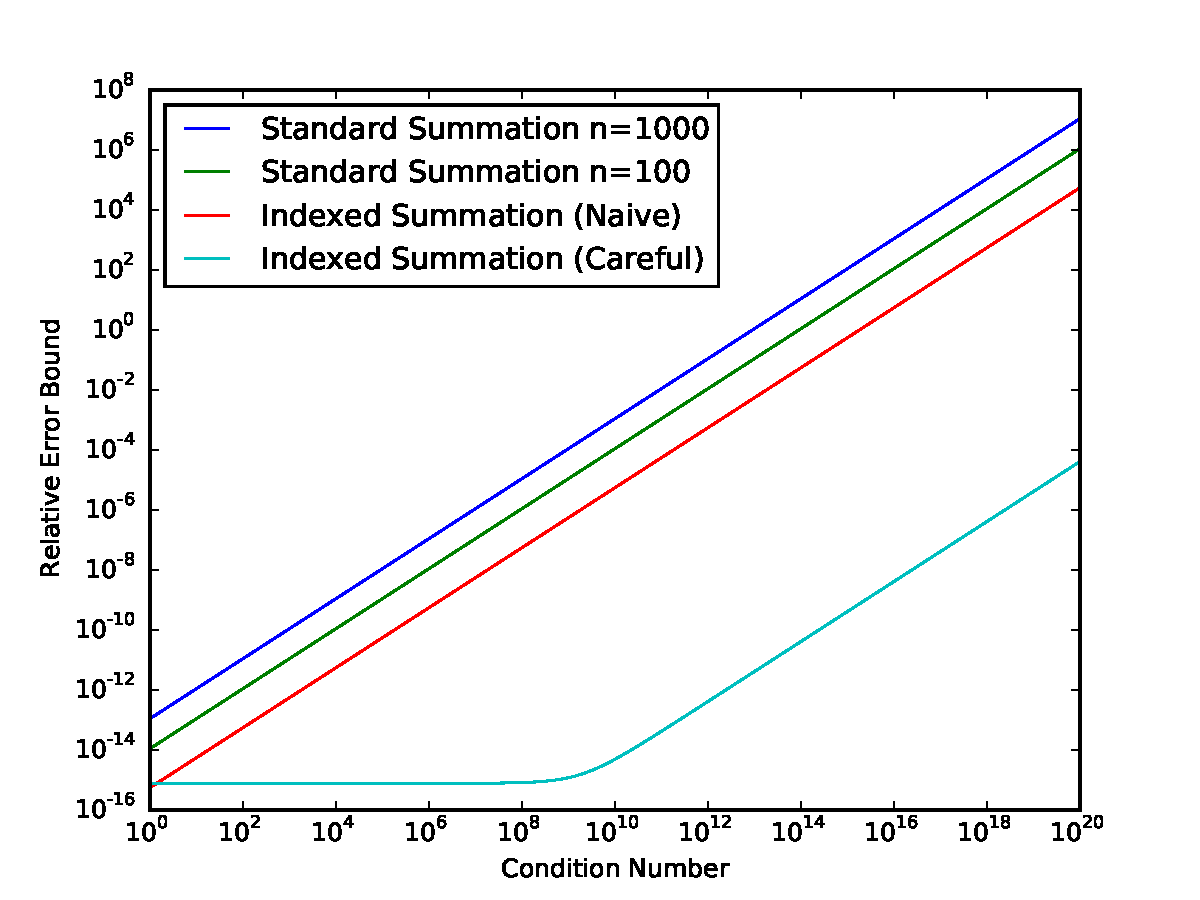
\includegraphics[width=\textwidth]{plots/errorcomparison.pdf}
\caption{Relative error bounds in calculating $|\sum \limits_{j = 0}^{n - 1}
x_j|$ for different condition numbers (which we define as $\frac{n \cdot \max
|x_j|)}{|\sum \limits_{j = 0}^{n - 1} x_j|}$) of the sum. It is assumed that we
sum using \texttt{double}, $K = 3$, and $W = 40$. ``Indexed Summation
(Careful)'' corresponds to \eqref{eq:errorapproxdup}. ``Indexed Summation
(Naive)'' corresponds to \eqref{eq:baderrorapproxdup}. ``Standard Summation''
corresponds to \eqref{eq:naiveerrorapproxdup} and due to a dependence on $n$
multiple error bounds are shown.}
\label{fig:conversionmotivation}
\end{center}
\end{figure}

    Consider a $K$-fold indexed type $Y$ of index $I$.
    As each value ${\mathcal{Y}_k}_P$ in a primary field ${Y_k}_P$ is represented by an offset from $1.5  \epsilon^{-1}  2^{a_{I + k}}$ and ${Y_k}_P \in (\epsilon^{-1}  2^{a_{I + k}}, 2  \epsilon^{-1}  2^{a_{I + k}})$, ${\mathcal{Y}_k}_P$ can be expressed exactly using an unnormalized floating point number ${\mathcal{Y}'_P}_k$ with an exponent of $a_{I + k} + p - 1$.
    As each carry field ${Y_k}_C$ is a count of renormalization adjustments later scaled by $0.25  \epsilon^{-1}  2^{a_{I + k}}$, ${\mathcal{Y}_k}_C$ can be expressed exactly using an unnormalized floating point number ${\mathcal{Y}'_k}_C$ with an exponent of $a_{I + k} + 2  p - 3$.

    First, we have $\exp({\mathcal{Y}'_k}_P) > \exp({\mathcal{Y}'_{k+1}}_P)$ and $\exp({\mathcal{Y}'_{k}}_C) > \exp({\mathcal{Y}'_{k+1}}_C)$ because $a_{I + k} > a_{I + k+1}$.

    Next, note that
    \begin{equation*}
      \exp({\mathcal{Y}'_k}_C) = a_{I + k} + 2  p - 3
    \end{equation*}

    and
    \begin{equation*}
      \exp({\mathcal{Y}'_{k - 1}}_P) = a_{I + k - 1} + p - 1 = a_{I + k} + W + p - 1
    \end{equation*}

    Therefore $\exp({\mathcal{Y}'_k}_C) > \exp({\mathcal{Y}'_{k - 1}}_P)$ because $W < p - 2$.

    Finally, note that
    \begin{equation*}
      \exp({\mathcal{Y}'_{k - 2}}_P) = a_{I + k - 1} + p - 1 = a_{I + k} + 2 W + p - 1
    \end{equation*}

    Therefore $\exp({\mathcal{Y}'_k}_C) < \exp({\mathcal{Y}'_{k - 2}}_P)$ because $2  W > p + 1$.

    Combining the above inequalities, we see that the exponents of all the ${\mathcal{Y}'_k}_P$ and ${\mathcal{Y}'_k}_C$ are distinct and can be sorted as follows:

    \begin{alignat*}{5}
    \exp({\mathcal{Y}'_0}_C) &> \exp({\mathcal{Y}'_1}_C) &&> \exp({\mathcal{Y}'_0}_P) &&> \exp({\mathcal{Y}'_2}_C) &&> \exp({\mathcal{Y}'_1}_P) &&> ... \\
    ... &> \exp({\mathcal{Y}'_k}_C) &&> \exp({\mathcal{Y}'_{k - 1}}_P) &&> \exp({\mathcal{Y}'_{k + 1}}_C) &&> \exp({\mathcal{Y}'_k}_P) &&> ... \\
    ... &> \exp({\mathcal{Y}'_{K - 2}}_C) &&> \exp({\mathcal{Y}'_{K - 3}}_P) &&> \exp({\mathcal{Y}'_{K - 1}}_C) &&> \exp({\mathcal{Y}'_{K - 2}}_P) &&> \exp({\mathcal{Y}'_{K - 1}}_P)
    \end{alignat*}


    These unnormalized floating point numbers may, for convenience of notation,
    be referred to in decreasing order of unnormalized exponent as $\gamma'_0,
    ..., \gamma'_{2  K - 1}$.

    We have just shown that
    \begin{equation}
      \exp(\gamma_0') > ... > \exp(\gamma_{2  K - 1}')
      \label{eq:gammadecreases}
    \end{equation}
    where $\gamma_j$ denotes the normalized representations of the $\gamma'_j$.
    It should be noted that $\gamma_j = \gamma'_j$ as real numbers and that
    $\exp(\gamma_j) \leq \exp(\gamma'_j)$.

    It should be noted that if $\gamma_j$ is a primary field, then either
    $\gamma_{j + 1}$ or $\gamma_{j + 2}$ is a primary field. If $\gamma_j$ is a
    carry field, then either $\gamma_{j + 1}$ or $\gamma_{j + 2}$ is a carry
    field (with the exception of $\gamma_{2  K - 3}$, but in this case we have
    \(
        \exp(\gamma_{2  K - 3})
        = a_{I + K - 1} + 2  p - 3 \geq a_{I + K - 1} + p + \lceil\frac{p + 1}{2}\rceil - 1
        = \exp(\gamma_{2  K - 1}) + \lceil\frac{p + 1}{2}\rceil
    \)
    ). Therefore, as $2  W > p + 1$, for all $j \in \{0, ..., 2
    K - 1\}$
    \begin{equation}
      \exp(\gamma_j') \geq \exp(\gamma_{j + 2}') + W \geq \exp(\gamma_{j + 2}') + \left\lceil\frac{p + 1}{2}\right\rceil
      \label{eq:gammadecreasesfast}
    \end{equation}

    It should be noted that the ${\mathcal{Y}'_k}_P$ and the
    ${\mathcal{Y}'_k}_C$ can be expressed exactly using floating point types of
    the same precision as ${Y_k}_P$ and ${Y_k}_C$ (except in the case of
    overflow, in which a scaled version may be obtained), and such exact
    floating point representations can be obtained using  \eqref{eq:pri} and
    \eqref{eq:car}.

    Now that we know how to obtain sorted, possibly scaled, fields in order of
    decreasing unnormalized exponent, we explain how to sum them while avoiding
    overflow. We will refer to the floating point type that we use to hold the
    sum during computation as the \textbf{intermediate} floating point type.
    Such a type must have at least as much precision and exponent range as the
    original floating point type.

    Notice that $|\gamma'_0| = |{\mathcal{Y}'_0}_C| < 2 \cdot 2^{\exp({\mathcal{Y}'_0}_C)} = 2 \cdot 2^{e_{\max} + 1 - W + 2  p - 3}$ and $\exp(\gamma'_0) > ... > \exp(\gamma'_{2  K - 1})$.  Therefore $|\gamma'_j| \leq 2^{e_{\max} - W + 2  p - 1 - j}$. The absolute value represented by an indexed type can therefore be bounded by

    \begin{equation}
      \label{eq:maxindexedvalue}
      \sum\limits_{j = 0}^{2  K - 1} |\gamma_j| < \sum\limits_{j = 0}^{2  K - 1} 2^{e_{\max} - W + 2  p - 1 - j} < \sum\limits_{j = 0}^{\infty} 2^{e_{\max} - W + 2  p - 1 - j} = 2^{e_{\max} - W + 2  p}
    \end{equation}

    If the intermediate floating point type has a maximum exponent greater than
    or equal to $e_{\max} - W + 2  p - 1$, then no special cases to guard
    against overflow are needed.

    Algorithm \ref{alg:conv2float} represents a conversion routine in such a case.

    \begin{samepage}
    \begin{alg}
      Convert $K$-fold indexed type $Y$ of index $I$ to floating point $x$.
      Here, $z$ is a floating point type with at least the original precision
      and maximum exponent $E_{\max}$ greater than $e_{\max} - W + 2  p$
      \begin{algorithmic}[1]
        \Function{ConvertIndexedToFloat}{K, x, Y}
          \State $z = {\mathcal{Y}_0}_C$
          \For{$k = 1 \To K - 1$}
            \State $z = z + {\mathcal{Y}_k}_C$
            \State $z = z + {\mathcal{Y}_{k - 1}}_P$
          \EndFor
          \State $z = z + {\mathcal{Y}_{K - 1}}_P$
          \State $x = z$ \label{alg:conv2float:conv}
        \EndFunction
      \end{algorithmic}
      \label{alg:conv2float}
    \end{alg}
    \end{samepage}

    Note that an overflow situation in Algorithm \ref{alg:conv2float} is
    reproducible as the fields in $Y$ are reproducible. $z$ is
    deterministically computed from the fields of $Y$, and the condition that
    $z$ overflows when being converted back to the original floating point type
    in line \ref{alg:conv2float:conv} is reproducible.

    If an intermediate floating point type with exponent greater than or equal
    to $e_{\max} - W + 2  p - 1$ is not available, the $\gamma_j$ must be
    scaled down by some factor during addition and the sum scaled back up when
    subsequent additions can no longer effect an overflow situation.

    If the scaled sum is to overflow, then its unscaled value will be greater
    than or equal to $2 \cdot 2^{e_{\max}}$ and it will overflow regardless of
    the values of any ${\mathcal{Y}_k}_P$ or ${\mathcal{Y}_k}_C$ with
    $|{\mathcal{Y}_k}_P| < 0.5 \cdot 2^{-\rho} 2^{e_{\max}}$ or
    $|{\mathcal{Y}_k}_C| < 0.5 \cdot 2^{-\rho}2^{e_{\max}}$ (where $\rho$ is
    the intermediate floating point type's precision). If the floating point
    sum has exponent greater than or equal to $e_{\max}$ these numbers are not
    large enough to have any effect when added to the sum. If the sum has
    exponent less than $e_{\max}$, then additions of these numbers cannot cause
    the exponent of the sum to exceed $e_{\max}$ for similar reasons.

    As the maximum absolute value of the true sum is strictly smaller than
    $2^{e_{\max} - W + 2 p}$, a sufficient scaling factor is $2^{2p-W-2}$,
    meaning that the maximum absolute value of the true scaled sum is
    strictly smaller $2 \cdot 2^{e_{\max} - 1}$ (and since it will be shown
    later that the computed sum is accurate to within a small factor of the
    true sum, the computed sum will stay strictly smaller than $2 \cdot
    2^{e_{\max}}$ and will not overflow.)

    When $\exp(\gamma'_j) < e_{\max} - \rho - 1$, the sum may be scaled back up
    and the remaining numbers added without scaling. Notice that no overflow
    can occur during addition in this algorithm. If an overflow is to occur, it
    will happen only when scaling back up. As the fields in the indexed type
    are reproducible, such an overflow condition is reproducible.

    If the sum is not going to overflow, then the smaller $y'_j$ must be added
    as unscaled numbers to avoid underflow.

    Algorithm \ref{alg:conv2floatoverflow} represents a conversion routine in such a case.

    \begin{samepage}
    \begin{alg}
      Convert a $K$-fold indexed type $Y$ of index $I$ to floating point $x$.
      Here, $z$ is a floating point number with precision $\rho > p$
      \begin{algorithmic}[1]
        \Function{ConvertIndexedToFloat}{K, x, Y}
          \State $k = 1$
          \While{$k \leq 2 K$ and $\exp(\gamma_k) \geq e_{\max} - \rho - 1$}
            \State $z = z + (\gamma_k / 2^{2 p - W - 2})$
            \State $k = k + 1$
          \EndWhile
          \State $z = z \cdot 2^{2 p - W - 2}$
          \While{$k \leq 2 K$}
            \State $z = z + \gamma_k$
            \State $k = k + 1$
          \EndWhile
          \State $x = z$
        \EndFunction
      \end{algorithmic}
      \label{alg:conv2floatoverflow}
    \end{alg}
    \end{samepage}

    If an indexed type is composed of \texttt{float}, then \texttt{double}
    provides sufficient precision and exponent to use as an intermediate type
    and Algorithm \ref{alg:conv2float} may be used to convert to a floating
    point number.  However, if an indexed type is composed of \texttt{double},
    many machines may not have any higher precision available. We therefore
    perform the sum using \texttt{double} as an intermediate type. As this does
    not extend the exponent range we must use Algorithm
    \ref{alg:conv2floatoverflow} for the conversion.

  \subsection{Error Bound}
    \label{sec:primitiveops_error}

    We first state and prove Theorem \ref{thm:mysortsum}, as it is critical in
    the error analysis of the algorithm. It should be noted that Theorem
    \ref{thm:mysortsum} is similar to that of Theorem 1 from \cite{sortsum},
    but requires less intermediate precision by exploiting additional structure
    of the input data.

    It is possible that future implementors may make modifications to the
    indexed type (adding multiple carry fields, changing the binning scheme,
    etc.) such that the summation of its fields cannot be reordered to satisfy
    the assumptions of Theorem \ref{thm:mysortsum}. In such an event,
    $\cite{sortsum}$ provides more general ways to sum the fields while still
    maintaining accuracy.
      \begin{samepage}
    \begin{thm}
      Given $n$ floating point numbers $f_0, \ldots, f_{n - 1}$ for which there
      exist (possibly unnormalized) floating point numbers $f'_0, \ldots, f'_{n -1}$
      of the same precision such that
      \begin{enumerate}
        \item $f_j = f'_j$ for all $j \in \{0, ..., n - 1\}$
        \item $\exp(f'_0) > ... > \exp(f'_{n - 1})$
        \item $\exp(f'_j) \geq \exp(f'_{j + 2}) + \lceil\frac{p + 1}{2}\rceil$ for all $j \in \{0, ..., n - 3\}$
      \end{enumerate}
      \label{thm:mysortsum}
      Let $S_0 = \overline{S_0} = f_0$, $S_j = S_{j - 1} + f_j$,
      and $\overline{S_j} = \fl(\overline{S_{j - 1}} + f_j)$ (assuming rounding to nearest)
      so that $S_{n - 1} = \sum \limits_{j = 0}^{n - 1} f_j$.
      Then in the absence of overflow and underflow we have
      \begin{equation*}
        \left|S_{n - 1} - \overline{S_{n - 1}}\right| < \frac{7\epsilon}{1 - 6\sqrt\epsilon}|S_{n - 1}| \approx 7 \epsilon |S_{n - 1}|
      \end{equation*}
    \end{thm}
    \end{samepage}

    \begin{proof}

      Throughout the proof, let $f_j = 0$ if $j > n - 1$ so that $S_{\infty} = S_{n - 1}$ and $\overline{S_{\infty}} = \overline{S_{n - 1}}$.

      Let $m$ be the location of the first error such that $S_{m - 1} = \overline{S_{m - 1}}$ and $S_{m} \neq \overline{S_{m}}$.

      If no such $m$ exists then the computed sum is exact ($S_{n - 1} = \overline{S_{n - 1}}$) and we are done.

      If such an $m$ exists, then because $\exp(f_0') > ... > \exp(f_m')$, $f_0, ..., f_m \in \ulp(f_m')\Z$. Thus, $S_m \in \ulp(f_m')\Z$.

      We now show $|S_m| > 2 \cdot 2^{\exp(f_m')}$. Assume for contradiction that $|S_m| \leq 2 \cdot 2^{\exp(f_m')}$. Because $S_m \in \ulp(f_m')\Z$, this would imply that $S_m$ is representable as a floating point number, a contradiction as $\overline{S_m} \neq S_m$. Therefore, we have
      \begin{equation}
        |S_m| > 2 \cdot 2^{\exp(f_m')}
        \label{eq:smbound}
      \end{equation}

      Because $\exp(f_m') > \exp(f_{m + 1}')$,
      \begin{equation}
        |f_{m + 1}| < 2\cdot2^{\exp(f_m' - 1)} = 2^{\exp(f_m')}
        \label{eq:smpbound}
      \end{equation}

      Because $\exp(f_m') \geq \exp(f_{m + 2}') + \lceil\frac{p + 1}{2}\rceil$ and $\exp(f_0') > ... > \exp(f_{n - 1}')$,
      \begin{align}
        \bigl|\sum \limits_{j = m + 2}^{n - 1} f_j\bigr| &\leq \sum \limits_{j = m + 2}^{n - 1} |f_j| < \sum \limits_{j = m + 2}^{n - 1} 2 \cdot 2^{\exp(f_j')} \leq \sum \limits_{j = m + 2}^{n - 1} 2 \cdot 2^{\exp(f_m') - \left\lceil\frac{p + 1}{2}\right\rceil - (m + 2 - j)} \nonumber \\
        &< \sum \limits_{j = 0}^{\infty} \left(2 \sqrt{\epsilon}\right)2^{\exp(f_m') - j} = \left(4\sqrt\epsilon\right)2^{\exp(f_m')}
        \label{eq:smppbound}
      \end{align}

      We can combine  \eqref{eq:smpbound} and \eqref{eq:smppbound} to obtain
      \begin{equation}
        \bigl|\sum\limits_{j = m + 1}^{n - 1} f_j\bigr| \leq \sum\limits_{j = m + 1}^{n - 1} |f_j| < 2^{\exp{f_m'}} + \left(4 \sqrt{\epsilon}\right) 2^{\exp(f_m')} = \left(1 + 4 \sqrt\epsilon \right)2^{\exp(f_m')}
        \label{eq:smsbound}
      \end{equation}

      By  \eqref{eq:smbound} and \eqref{eq:smsbound},
      \begin{align}
        |S_{n-1}| & = \bigl|\sum\limits_{j = 0}^{n - 1} f_j\bigr| \geq \bigl|\sum\limits_{j = 0}^{m} f_j\bigr| - \bigl|\sum\limits_{j = m + 1}^{n - 1} f_j\bigr| = |S_m| - \bigl|\sum\limits_{j = m + 1}^{n - 1} f_j\bigr| \nonumber \\
        & \geq 2 \cdot 2^{\exp(f_{m}')} - \left(1 + 4 \sqrt\epsilon\right) 2^{\exp(f_m')} = \left(1 - 4 \sqrt\epsilon\right) 2^{\exp(f_m')}
        \label{eq:sbound}
      \end{align}

      By  \eqref{eq:sbound} and \eqref{eq:smppbound},
      \begin{equation}
        \bigl|\sum \limits_{j = m + 2}^{n - 1} f_j\bigr| < \left(4 \sqrt{\epsilon}\right) 2^{\exp(f_m')} \leq \frac{4 \sqrt\epsilon}{1 - 4  \sqrt\epsilon}\bigl|\sum\limits_{j = 0}^{n - 1}f_j\bigr|
        \label{eq:smpprelsbound}
      \end{equation}

      By  \eqref{eq:sbound} and \eqref{eq:smsbound},
      \begin{equation}
        \bigl|\sum\limits_{j = m + 1}^{n - 1}f_j\bigr| \leq \sum\limits_{j = m + 1}^{n - 1}|f_j| \leq \left(1 + 4  \sqrt\epsilon\right)2^{\exp(f_m')}\leq \frac{1 + 4  \sqrt\epsilon}{1 - 4  \sqrt\epsilon}\bigl|\sum\limits_{j = 0}^{n - 1}f_j\bigr|
        \label{eq:smsrelsbound}
      \end{equation}

      And by \eqref{eq:sbound} and \eqref{eq:smsrelsbound},
      \begin{equation}
        |S_m| \leq \bigl|\sum\limits_{j = 0}^{n - 1}f_j\bigr| + \bigl|\sum\limits_{j = m + 1}^{n - 1} f_j\bigr|
            \leq \left(1 + \frac{1 + 4\sqrt\epsilon}{1 - 4\sqrt\epsilon}\right)\bigl|\sum_{j = 0}^{n - 1}f_j\bigr|
            = \frac{2}{1 - 4  \sqrt\epsilon}\bigl|\sum\limits_{j = 0}^{n - 1}f_j\bigr|
        \label{eq:smrelsbound}
      \end{equation}

      By definition, $\overline{S_{m+4}}$ is the computed sum of
      $\overline{S_m}$, $f_{m+1}, \ldots, f_{m+4}$ using the standard recursive summation technique.
      According to \cite[Equation 1.2, 2.4]{higham}
      \begin{align*}
          \bigl|\overline{S_m} + \sum_{j=m+1}^{m+4}f_j - \overline{S_{m+4}}\bigr|
          & \leq \frac{4\epsilon}{1-4\epsilon} \left|\overline{S_m} + f_{m+1}\right| + \frac{3\epsilon}{1-3\epsilon} \sum_{j=m+2}^{m+4}|f_j| \\
          & \leq \frac{4\epsilon}{1-4\epsilon} \bigl(\left|\overline{S_m} - S_m\right| + |S_m + f_{m+1}|\bigr)
              + \frac{3\epsilon}{1-3\epsilon} \sum_{j=m+2}^{n-1}|f_j|.
      \end{align*}
      Since $S_{n-1} = S_m + f_{m+1} + \sum_{j=m+2}^{n-1} f_j$, we have
      \begin{equation*}
          |S_m + f_{m+1}|
          = \bigl|S_{n-1} - \sum_{j=m+2}^{n-1}f_j\bigr|
          \leq |S_{n-1}| + \sum_{j=m+2}^{n-1} |f_j|
      \end{equation*}
      Therefore
      \begin{equation*}
          \bigl|\overline{S_m} + \sum_{j=m+1}^{m+4}f_j - \overline{S_{m+4}}\bigr|
          \leq \frac{4\epsilon}{1-4\epsilon} \left|S_m - \overline{S_m}\right|
          + \frac{4\epsilon}{1-4\epsilon} |S_{n-1}|
          + \frac{7\epsilon}{1-4\epsilon} \sum_{j=m+2}^{n-1}|f_j|.
      \end{equation*}
      Using the triangle inequality we have
      \begin{align*}
      \left|S_{m+4} - \overline{S_{m+4}}\right|
          & = \bigl|S_m + \sum_{j=m+1}^{m+4}f_j - \overline{S_{m+4}}\bigr|
          \leq \left|S_m - \overline{S_m} \right| + \bigl|\overline{S_m} + \sum_{j=m+1}^{m+4}f_j - \overline{S_{m+4}} \bigr| \\
          & \leq \left(1 + \frac{4\epsilon}{1-4\epsilon}\right) \left|S_m - \overline{S_m}\right| + \frac{4\epsilon}{1-4\epsilon} |S_{n-1}|
                  + \frac{7\epsilon}{1-4\epsilon} \sum_{j=m+2}^{n-1}|f_j| \\
          & \leq \frac{1}{1-4\epsilon} \epsilon |S_m| + \frac{4\epsilon}{1-4\epsilon} |S_{n-1}|
                  + \frac{7\epsilon}{1-4\epsilon} \sum_{j=m+2}^{n-1}|f_j| \\
          & \leq \frac{\epsilon}{1-4\epsilon} \left(|S_m| + 4 |S_{n-1}|
                  + 7 \sum_{j=m+2}^{n-1}|f_j|\right).
      \end{align*}
      and by \eqref{eq:smrelsbound} and \eqref{eq:smpprelsbound},
      \begin{align}
      \left|S_{m+4} - \overline{S_{m+4}}\right|
          & \leq \frac{\epsilon}{1-4\epsilon}
              \left(
                  \frac{2}{1-4\sqrt{\epsilon}} |S_{n-1}|
                  + 4 |S_{n-1}|
                  + 7 \frac{4\sqrt{\epsilon}}{1-4\sqrt{\epsilon}} |S_{n-1}|
              \right) \nonumber \\
          & \leq \frac{\epsilon}{1-4\epsilon} \left(\frac{6+12\sqrt{\epsilon}}{1-4\sqrt{\epsilon}} |S_{n-1}|\right)
              = \frac{6\epsilon }{(1-2\sqrt{\epsilon})(1-4\sqrt{\epsilon})} |S_{n-1}| \nonumber \\
          & < \frac{6\epsilon}{1-6\sqrt{\epsilon}} |S_{n-1}|
          \label{eq:smfiveerror}
      \end{align}

      Notice that
      \begin{equation*}
        \exp(f_m') \geq \exp(f_{m + 2}') + \left\lceil\frac{p+ 1}{2}\right\rceil \geq \exp(f_{m + 4}') + 2  \left\lceil\frac{p + 1}{2}\right\rceil > \exp(f_{m + 5}')+ 2  \left\lceil\frac{p+ 1}{2}\right\rceil
      \end{equation*}
      Therefore,
      \begin{equation}
        \exp(f_m') \geq \exp(f_{m + 5}') + p + 2
        \label{eq:fmfiveexp}
      \end{equation}

      Because $\exp(f_0') > ... > \exp(f_{n - 1}')$, \eqref{eq:fmfiveexp} yields
      \begin{equation}
        \bigl|\sum\limits_{j = m + 5}^{n - 1} f_j\bigr| \leq \sum\limits_{j = m + 5}^{n - 1} |f_j| < \sum\limits_{j = m + 5}^{n - 1} 2 \cdot 2^{\exp(f_m') - p - 2 - (j - (m + 5))} < \sum\limits_{j = 0}^{\infty} 2^{\exp(f_m') - p - 1 - j} = \epsilon 2^{\exp(f_m')}
        \label{eq:boundfmfivesum}
      \end{equation}

      Using \eqref{eq:sbound} and \eqref{eq:boundfmfivesum},
      \begin{equation}
        \bigl|\sum\limits_{j = m + 5}^{n - 1} f_j\bigr| \leq \sum\limits_{j = m + 5}^{n - 1} |f_j| < \frac{\epsilon}{1 - 4  \sqrt\epsilon}|S_{n - 1}|
        \label{eq:relsboundfmfivesum}
      \end{equation}

      By \eqref{eq:smfiveerror} and \eqref{eq:relsboundfmfivesum}
      \begin{align}
        \left|S_{n-1} - \overline{S_{m+4}}\right|
        & \leq |S_{n-1} - S_{m+4}| + \left|S_{m+4} - \overline{S_{m+4}}\right| \nonumber \\
        & \leq \bigl|\sum_{j=m+5}^{n-1} f_j\bigr| + \frac{6\epsilon}{1-6\sqrt{\epsilon}} |S_{n-1}| \nonumber \\
        & \leq \frac{\epsilon}{1 - 4 \sqrt\epsilon}|S_{n-1}| + \frac{6\epsilon}{1-6\sqrt{\epsilon}} |S_{n-1}| \nonumber \\
        & <  \frac{7\epsilon}{1-6\sqrt{\epsilon}} |S_{n-1}|.
        \label{eq:smfiveerror-1}
      \end{align}

      When combined with \eqref{eq:sbound} this gives
      \begin{align*}
        \left|\overline{S_{m+4}}\right|
        & \geq \left(1-\frac{7 \epsilon}{1-6\sqrt{\epsilon}}\right) |S_{n-1}| \\
        & > \left(1-\frac{7 \epsilon}{1-6\sqrt{\epsilon}}\right) \left(1-4\sqrt{\epsilon}\right) 2^{\exp(f'_m)} \\
        & > \left(1-4\sqrt{\epsilon} - \frac{7 \epsilon \left(1-4\sqrt{\epsilon}\right)}{1-6\sqrt{\epsilon}}\right) 2^{\exp(f'_m)}
      \end{align*}

      which, assuming $\epsilon \ll 1$, can be simplified to
      \begin{equation}
        \left|\overline{S_{m + 4}}\right| > 2^{\exp(f_m') - 1}
        \label{eq:minsmfoursimple}
      \end{equation}

      Using  \eqref{eq:fmfiveexp}, for all $j \geq m + 5$ we have
      \begin{equation}
        |f_j| < 2 \cdot 2^{\exp(f_j')} \leq 2 \cdot 2^{\exp(f_m') - p - 2} = \epsilon \cdot 2^{\exp(f_m') - 1}
        \label{eq:maxfmfive}
      \end{equation}

      And by \eqref{eq:maxfmfive} and \eqref{eq:minsmfoursimple}, all additions
      after $f_{m + 4}$ have no effect (since we are rounding to nearest)
      and we have $\overline{S_{n-1}} = \overline{S_{m+4}}$.
      This, together with \eqref{eq:smfiveerror-1}, implies
      \begin{equation*}
        \left|S_{n-1} - \overline{S_{n-1}}\right| < \frac{7\epsilon}{1-6\sqrt{\epsilon}} |S_{n-1}|
      \end{equation*}
      The proof is complete.
    \end{proof}

    Consider the $K$-fold indexed sum $Y$ of floating point numbers $x_0, \ldots, x_{n - 1}$.
    We denote the true sum $\sum \limits_{j = 0}^{n - 1} x_j$ by $T$, the true
    value of the indexed sum as obtained using \eqref{eq:indexedvalue} by
    $\mathcal{Y}$, and the floating point approximation of $\mathcal{Y}$
    obtained using an appropriate algorithm from Section
    \ref{sec:primitiveops_convert} by $\overline{\mathcal{Y}}$.

    \cite{repsum} discusses the absolute error $|T - \mathcal{Y}|$ but does not
    give a method to construct $\overline{\mathcal{Y}}$ and therefore no error
    bound $|T - \overline{\mathcal{Y}}|$ on the final floating point answer
    was given. Here we extend the error bound of \cite{repsum} all the way to
    the final return value of the algorithm.

    %It has been shown in \cite{repsum} that
    Let $I$ be the index of $Y$, which is also the index of $\max|x_j|$,
    so that $2^{b_I} > \max|x_j| \geq 2^{a_I}$.
    Therefore for all $i < I$ the slice of any $x_j$ in bin $i$ is $d(x_j, i) = 0$.
    The index of the smallest bin of $Y$ is $I + K - 1$.
    According to Theorem~\ref{thm:dround}, we have
    \begin{align*}
        |x_j - \sum_{i=I}^{I + K -1} d(x_j,i)|
            & = |x_j - \sum_{i=0}^{I + K - 1} d(x_j,i)|
            \leq 2^{a_{I + K -1}} 
            = 2^{a_I - (K-1)W} \\
            & \leq 2^{W(1-K)} \max|x_j|. 
    \end{align*}

    Since the summation in each bin $Y_i$ is exact, we have
    \begin{align}
        |T - \mathcal{Y}| & = |\sum_{j=0}^{n-1} x_j - \sum_{i=I}^{I+K-1} \sum_{j=0}^{n-1} d(x_j, i)|
            = |\sum_{j=0}^{n-1} (x_j - \sum_{i=I}^{I+K-1} d(x_j,i))| \nonumber \\
            & \leq n 2^{W(1-K)} \max|x_j|.
            \label{eq:repboundnaive}
    \end{align}

    However, this bound does not consider underflow. By
    \eqref{eq:droundunderflow}, a small modification yields a bound that
    considers underflow
    \begin{equation}
      \label{eq:repbound}
      |T - \mathcal{Y}| < n \cdot \max\bigl(2^{W  (1 - K)} \max|x_j|, 2^{e_{\min} - 1}\bigr)
    \end{equation}

    By  \eqref{eq:gammadecreases} and \eqref{eq:gammadecreasesfast},
    Theorem \ref{thm:mysortsum} applies to yield
    \begin{equation*}
      \left|\mathcal{Y} - \overline{\mathcal{Y}}\right| < \frac{7\epsilon}{1 - 6\sqrt\epsilon}|\mathcal{Y}|
    \end{equation*}

    By the triangle inequality
    \begin{equation*}
      |\mathcal{Y}| \leq |T| + |T - \mathcal{Y}| < n \cdot \max\bigl(2^{W(1-K)}  \max|x_j|, 2^{e_{\min} - 1}\bigr) + |T|
    \end{equation*}

    The above results can be used to obtain  \eqref{eq:error}, the absolute
    error of the floating point approximation of an indexed sum $|T - \overline{\mathcal{Y}}|$.
    \begin{align}
      \left|T - \overline{\mathcal{Y}}\right| &\leq |T - \mathcal{Y}| + \left|\mathcal{Y} - \overline{\mathcal{Y}}\right| \nonumber \\
      &< n \cdot \max\bigl(2^{W  (1 - K)}  \max|x_j|, 2^{e_{\min} - 1}\bigr) + \frac{7\epsilon}{1 - 6\sqrt\epsilon} |\mathcal{Y}| \nonumber \\
      &< n \cdot \max\bigl(2^{W  (1 - K)}  \max|x_j|, 2^{e_{\min} - 1}\bigr) \nonumber \\
      &+ \frac{7\epsilon}{1 - 6\sqrt\epsilon} \Bigl(n \cdot \max\bigl(2^{W  (1 - K) - 1}  \max|x_j|, 2^{e_{\min} - 1}\bigr) + |T|\Bigr) \nonumber \\
      &< \left(1 + \frac{7\epsilon}{1 - 6\sqrt\epsilon}\right) \Bigl(n \cdot \max\bigl(2^{W (1 - K)} \max|x_j|, 2^{e_{\min} - 1}\bigr)\Bigr) + \frac{7\epsilon}{1 - 6\sqrt\epsilon} |T|
      \label{eq:error}
    \end{align}

    Equation \eqref{eq:error} can be approximated as \eqref{eq:errorapprox}:
    \begin{align}
      \left|T - \overline{\mathcal{Y}}\right| &< \left(1 + \frac{7\epsilon}{1 - 6\sqrt\epsilon}\right) \Bigl(n \cdot \max\bigl(2^{W (1 - K)} \max|x_j|, 2^{e_{\min} - 1}\bigr)\Bigr) + \frac{7\epsilon}{1 - 6\sqrt\epsilon} |T| \nonumber \\
    &\approx n 2^{W  (1 - K)} \max|x_j| + 7  \epsilon |T|
      \label{eq:errorapprox}
    \end{align}

    A perhaps more useful mathematical construction is the error expressed
    relative to the result $\overline{\mathcal{Y}}$, and not the theoretical
    sum $T$. Again by the triangle inequality,
    \begin{equation*}
      |\mathcal{Y}| \leq \left|\overline{\mathcal{Y}}\right| + \left|\mathcal{Y} - \overline{\mathcal{Y}}\right|
    \end{equation*}

    Applying the bound on $|\mathcal{Y} - \overline{\mathcal{Y}}|$ yields
    \begin{equation*}
      |\mathcal{Y}| < \left|\overline{\mathcal{Y}}\right| + \frac{7\epsilon}{1 - 6\sqrt\epsilon}|\mathcal{Y}|
    \end{equation*}

    After simplification,
    \[
      |\mathcal{Y}| < \left(\frac{1}{1 - \frac{7\epsilon}{1 - 6\sqrt\epsilon}}\right)  \left|\overline{\mathcal{Y}}\right| \nonumber 
      = \frac{1 - 6 \sqrt\epsilon}{1 - 6 \sqrt \epsilon - 7\epsilon}  \left|\overline{\mathcal{Y}}\right|.
    \]

    The above results can be used to obtain  \eqref{eq:error2}, the absolute
    error of the floating point approximation of an indexed sum $|T -
    \overline{\mathcal{Y}}|$.
    \begin{align}
      \left|T - \overline{\mathcal{Y}}\right| &\leq |T - \mathcal{Y}| + \left|\mathcal{Y} - \overline{\mathcal{Y}}\right| \nonumber \\
      &< n \cdot \max\bigl(2^{W(1-K)}  \max|x_j|, 2^{e_{\min} - 1}\bigr) + \frac{7\epsilon}{1 - 6\sqrt\epsilon}|\mathcal{Y}| \nonumber \\
      &< n \cdot \max\bigl(2^{W(1-K)}  \max|x_j|, 2^{e_{\min} - 1}\bigr) + \frac{7\epsilon}{1 - 6\sqrt\epsilon}\left(\frac{1 - 6 \sqrt\epsilon}{1 - 6 \sqrt \epsilon - 7\epsilon}\left|\overline{\mathcal{Y}}\right|\right) \nonumber \\
      &= n \cdot \max\bigl(2^{W(1-K)}  \max|x_j|, 2^{e_{\min} - 1}\bigr) + \frac{7\epsilon}{1 - 6 \sqrt \epsilon - 7\epsilon}\left|\overline{\mathcal{Y}}\right|
      \label{eq:error2}
    \end{align}

    Equation \eqref{eq:error2} can be approximated as \eqref{eq:error2approx},
    which is nearly equal to bound \eqref{eq:errorapprox}:
    \begin{align}
      |T - \overline{\mathcal{Y}}| &< n \cdot \max\bigl(2^{W(1-K)}  \max|x_j|, 2^{e_{\min} - 1}\bigr) + \frac{7\epsilon}{1 - 6 \sqrt \epsilon - 7\epsilon}  \left|\overline{\mathcal{Y}}\right| \nonumber \\
      &\approx n  2^{W(1 - K)} \max|x_j|+ 7 \epsilon \left|\overline{\mathcal{Y}}\right|
      \label{eq:error2approx}
    \end{align}

    We can compare  \eqref{eq:errorapprox} to the error bound obtained if the
    accumulator fields were summed without extra precision. In this case, only
    the standard summation bound from \cite{higham} would apply and the
    absolute error would be bounded by
    \begin{equation*}
    n \cdot \max\bigl(2^{W(1-K)}  \max|x_j|, 2^{e_{\min} - 1}\bigr) + \left(\frac{(2  K - 1)  \epsilon}{1 - (2  K - 1)  \epsilon}\right)  \sum\limits_0^{2  K - 1}|\gamma_j|
    \end{equation*}
    which is approximately bounded by
    \begin{equation}
    n \cdot \max|x_j| \bigl(2^{W(1-K)} + (2  K - 1)  \epsilon\bigr)
    \label{eq:baderrorapprox}
    \end{equation}

    This is not as tight a bound as \eqref{eq:errorapprox}, and grows linearly
    as the user increases $K$ in an attempt to increase accuracy.

  \subsection{Limits}
    \label{sec:primitiveops_limits}
    As discussed previously, for a $K$-fold indexed type the minimum $K$
    accepted by ReproBLAS is 2. The maximum useful $K$ is
    $\lfloor(e_{\max} - e_{\min} + p - 1)/W\rfloor$,
    as this covers all of the bins.

    As discussed in \cite{repsum}, $W < p - 2$. As discussed in section
    \ref{sec:indexed_overflow}, $2 W > p + 1$.

    ReproBLAS uses the values $W = 40$ for indexed \texttt{double} and $W = 13$
    for indexed \texttt{float}. $W$ is available as the \texttt{XIWIDTH} macro.

    As discussed in section \ref{sec:indexed_underflow_gradual}, the input is
    rounded at best to the nearest $2^{e_{\min} - 1}$

    As absolute value of individual quantities added to ${Y_k}_P$ are not in
    excess of $2^{b_{I + k}}$, a maximum of $0.25\epsilon^{-1}2^{-W}$ elements
    may be deposited into ${Y_k}_P$ between renormalizations, as discussed in
    section \ref{sec:primitiveops_renormalize}. For indexed \texttt{double}
    this number is $2^{11}$, whereas for indexed \texttt{float} this number is
    $2^9$. This number is supplied programmatically using the
    \texttt{XIENDURANCE} macro.

    By \eqref{eq:totalfreq}, an indexed sum is capable of representing the sum
    of at least $0.25\epsilon^{-1}2^{-W}  (\epsilon^{-1} - 1) \approx 2^{2  p - W - 2}$
    floating point numbers. For indexed \texttt{double} this number is
    almost $2^{64}$, whereas for indexed \texttt{float} this number is almost
    $2^{33}$. This number is supplied programmatically using the
    \texttt{XICAPACITY} macro.

    The indexed types provided by ReproBLAS will, when used correctly, avoid intermediate overflow.


\section{Interface}
  \subsection{Section Summary}
  \subsection{Fold}
  \subsection{Complex Types}
  \subsection{Naming Conventions}
  \subsection{Build System}
\section{indexed.h}
  \subsection{Section Summary}
  \subsection{Types}
  \subsection{Functions}
    \subsubsection{xixadd}
    \subsubsection{xixiadd}
    \subsubsection{xscale}
    \subsubsection{xixiaddsq}
\section{idxdBLAS.h}
  \label{sec:idxdBLAS}
  \subsection{Section Summary}
  \subsection{Functions}
    \subsubsection{xixdot}
    \subsubsection{xixnrm2}
    \subsubsection{xixgemv}
    \subsubsection{xixgemm}
  \subsection{Optimization}
    Due to the proportion of time spent in the deposit routine, optimization of the deposit routine was prioritized. In the event that multiple $x$ need to be added to $Y$, the deposit routine can be vectorized by accumulating the $x$ in multiple copies of $Y$. The number of copies of $Y$ to make, $c$, and the number of unrolled loop iterations, $u$ are tuning parameters.
\section{repBLAS.h}
  \subsection{Section Summary}
\section{idxdMPI.h}
  \subsection{Section Summary}
  \subsection{Types}
  \subsection{Functions}
    \subsubsection{XIXIREDUCE}


\section{Applications}
  \subsection{Section Summary}
  \subsection{Parallel Reproducible Dot Product}
  \subsection{Parallel Reproducible Vector Norm}
  \subsection{Parallel Reproducible Matrix-Vector Multiply}
  \subsection{Parallel Reproducible Matrix-Matrix Multiply}


\bibliographystyle{plain}
\bibliography{biblio}

%\begin{thebibliography}{9}
%  \bibitem{repsum}
%    Demmel, James, and Hong Diep Nguyen. Parallel Reproducible Summation. IEEE Transactions on Computers, 2014.
%  \bibitem{ieee754}
%    IEEE Standard for Floating-Point Arithmetic, IEEE Std 754-2008 , vol., no., pp.1,70, Aug. 29 2008
%  \bibitem{c89}
%    ANSI/ISO 9899-1990 American National Standard for Programming Languages - C, section 6.1.2.5
%  \bibitem{higham}
%    Higham, Nicholas J. The accuracy of floating point summation. SIAM Journal on Scientific Computing 14, no. 4 (1993): 783-799.
%  \bibitem{sortsum}
%    Demmel, James W., and Yozo Hida. Accurate floating point summation. Computer Science Division, University of California, 2002.
%  %\bibitem{doubledouble}
%  %  Hida, Yozo, Xiaoye S. Li, and David H. Bailey. Quad-double arithmetic: Algorithms, implementation, and application. 15th IEEE Symposium on Computer Arithmetic, 2000.
%\end{thebibliography}
\end{document}
